\subsubsection{Zur Diskussion der modernen Bibliothek in der
Architekturpresse}\label{zur-diskussion-der-modernen-bibliothek-in-der-architekturpresse}

In der \emph{Revue générale de l'architecture et des travaux publics}
erschien im Jahr 1849 ein Beitrag des Herausgebers und Architekten César
Daly (1811-1894) über öffentliche Bibliotheken. (Abb. 1) Das Versprechen
der öffentlichen, für jeden zugänglichen Bibliothek, wie sie im 19.
Jahrhundert als Teil des staatlichen Erziehungs- und Bildungswesens
Verbreitung fand, scheint groß.\footnote{Wurden Hof-, Universitäts- und
  Klosterbibliotheken schon vor dem 19. Jahrhundert der Öffentlichkeit
  zugänglich gemacht, so erfolgte dies in der Regel mit deutlichen
  Einschränkungen hinsichtlich des Nutzerkreises, der Ausleihe und der
  Öffnungszeiten. Erst im 19. Jahrhundert, im Zuge des sich
  entwickelnden staatlichen Bildungs- und Erziehungswesens, kommt es zur
  Einrichtung und administrativen Regelung von öffentlichen Bibliotheken
  im heutigen Sinn.} Als Institution des Wissens und der Belehrung
vermag sie Daly zufolge auch noch das ungestümste Temperament zu zügeln,
Eisenschwerter in solche des Wortes zu verwandeln, die Augen der Pracht
der Natur, das Herz gegenüber den süßesten und nobelsten Gefühlen zu
öffnen, den Verstand zu nähren, damit er über das Licht des Schönen und
Guten am Wahren partizipiere.\footnote{César Daly, \enquote{Des
  bibliothèques publiques}, in: \emph{Revue générale de l'architecture
  et des travaux publics}, tome 8 (1849-50), S. 415-437, hier S. 415.}
Kurz, die öffentliche Bibliothek verspricht sowohl Gemüts- als auch
Verstandesbildung. Sie erweist sich als eines der wichtigsten
Instrumente allgemeiner Bildung.

\begin{figure}[htbp]
\centering
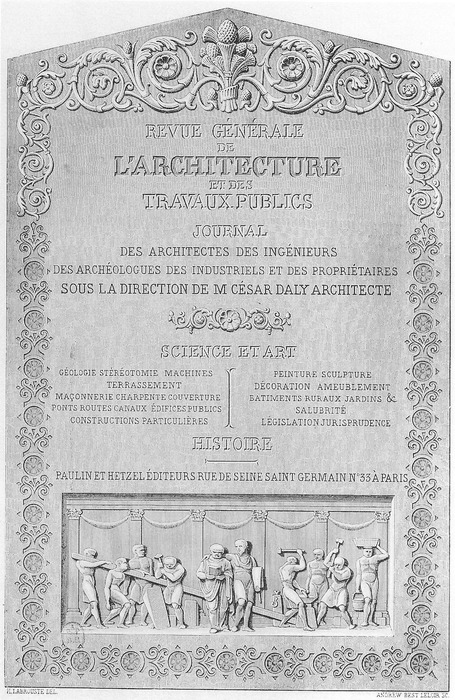
\includegraphics{img/wagner-1.jpg}
\caption*{Abb. 1: Frontispiz der \emph{Revue générale d'architecture et
des travaux publics}, tome 1, 1840.}
\end{figure}

Auf der Grundlage statistischer Erhebungen, die im 19. Jahrhundert zu
einem bedeutenden Planungs- und Steuerungsinstrument wurden, schließt
sich dieser Lobrede auf die öffentliche Bibliothek eine Übersicht über
Anzahl und Verbreitung bereits bestehender Bibliotheken in Frankreich
und anderen Ländern an. Mit 107 öffentlichen Bibliotheken, sieben davon
in Paris, kommen in Frankreich auf eine Bibliothek im Durchschnitt
336.448 Einwohner. Frankreich liegt damit im Vergleich zu anderen
europäischen Ländern und den Vereinigten Staaten an hinterer Stelle. Bei
der hypothetischen Pro-Kopf-Versorgung mit Büchern und anderen
Druckerzeugnissen schneiden die Toskana, Sachsen und Bayern am besten
ab. Doch nicht nur die statistisch erwiesene Unterversorgung der
Bevölkerung mit Literatur im weitesten Sinne\footnote{Im weitesten Sinne
  insofern, als die Bibliotheksbestände bis weit in das 19. Jahrhundert
  hinein mit anderen Objektsammlungen verquickt waren.} erweist sich als
problematisch und ruft den Architekten als Entwerfer und Erbauer von
Bibliotheken auf den Plan. Besonderer Handlungsbedarf besteht für Daly
bereits hinsichtlich der vorhandenen 107 Bibliotheken des Landes, denn
eigentlich handelt es sich mehr um Lagerräume von Buch- und
Handschriftenbeständen, die vielfach noch mit Münzen, Antiken und
Gemälden vermengt sind, und damit um Einrichtungen, die für Daly halb
Buchladen, halb Altwarenhändler sind.\footnote{Vgl. Daly, Bibliothèques
  publiques, S. 416.} Eine Ausnahme stellt für ihn lediglich die von
Henri Labrouste (1801-1875) entworfene Bibliothek
\emph{Sainte-Geneviève} dar, die im Jahr 1849 kurz vor ihrer
Fertigstellung stand.\footnote{Eine etwas ausführlichere Würdigung
  erfährt die Bibliothek \emph{Sainte-Geneviève} im zehnten Band der
  \emph{Revue générale de l'architecture et des travaux publics} (1852),
  S. 379-384.}

Mit der öffentlichen Bibliothek verhält es sich Daly zufolge genauso wie
mit den anderen neuen Bauaufgaben des 19. Jahrhunderts, insbesondere mit
den Bahnhöfen und den Eisenbahnstationen: die an der \emph{École des
beaux-arts} ausgebildeten Architekten seien auf sie, im Gegensatz zu den
Ingenieuren der technischen Hochschulen, in keiner Weise vorbereitet.
Wenn das historische Bild auch etwas anders ausfällt, tatsächlich
bleiben es die Architekten der Akademien, auf die die wichtigsten
Bibliotheksentwürfe und -bauten des 19. Jahrhunderts zurückgehen, dann
zeigt das die in der ersten Hälfte des 19. Jahrhunderts noch vollkommen
offene Frage, wie die moderne öffentliche Bibliothek in
architektonischer Hinsicht auszusehen hat. Denn welche Art von Gebäude
kann ihr nicht nur in ästhetischer und symbolischer, sondern auch in
funktionaler Hinsicht entsprechen? Ein Aspekt, der sowohl von Seiten der
Architektur als auch von Seiten der sich professionalisierenden
Bibliothekare in der ersten Jahrhunderthälfte zusehends in den
Vordergrund rückt. Wie nach ihm auch andere Architekten\footnote{Vgl.
  hierzu etwa Léonce Reynaud, \emph{Traité d'architecture, contenant des
  notions générales sur les principes de la construction et sur
  l'histoire de l'art}, deuxième partie: \enquote{Édifices}, Paris 1858,
  S. 381-388.} holt sich Daly Rat bei Léon de Laborde (1807-1869), der
vier Jahre zuvor in mehreren Briefen die kontrovers geführte Diskussion
um einen möglichen Abriss des Palais Mazarin beziehungsweise einen
Neubau der \emph{Bibliothèque royale}\footnote{Die \emph{Bibliothèque
  royale} wurde im Zuge der Französischen Revolution 1790 in
  \emph{Bibliothèque nationale} umbenannt, um während des zweiten
  Kaiserreiches zur \emph{Bibliothèque imperiale} zu werden. Danach trug
  sie wieder den Namen \emph{Bibliothèque nationale}. Vorliegend wird
  der Einfachheit halber durchgängig der historische Name
  \emph{Bibliothèque royale} verwendet.} aufgegriffen und eine kurze
Geschichte des Bibliotheksbaus mit einem Schwerpunkt auf dem 17. bis 19.
Jahrhundert vorgelegt hatte.\footnote{Zu diesen Briefen zählen der
  erste: \emph{De l'organisation des bibliothèques dans Paris. La
  Bibliothèque Royale occupe le centre topographique et intellectuel de
  la ville de Paris,} Paris 1845, in dem sich Laborde mit den
  verschiedenen zur Diskussion stehenden Standorten der Königlichen
  Bibliothek kritisch auseinandersetzt, der zweite über die
  entsprechenden Entwürfe: \emph{De l'organisation des bibliothèques
  dans Paris. Revue critique des projets présentés pour le déplacement
  de la Bibliothèque Royale}, der vierte mit einem historischen Abriss
  über den Palais Mazarin sowie städtische und ländliche Wohnhäuser des
  17. Jahrhunderts: \emph{De l'organisation des bibliothèques dans
  Paris. Le Palais Mazarin et les habitations de ville et de campagne au
  XVIIe siècle}, Paris 1845, der zugleich über die verschiedenen
  Ausgaben des sechsten Jahrganges der \emph{Revue générale de
  l'architecture et des travaux publics} abgedruckt wird, sowie der
  achte: \emph{De l'organisation des bibliothèques dans Paris. Étude sur
  la construction des bibliothèques}, Paris 1845, mit einem historischen
  Abriss der Bibliotheksarchitektur. Von den insgesamt zwölf geplanten
  Briefen sind nur diese vier erschienen. Vgl. hierzu auch Peter Prohl,
  \enquote{Vorwort}, in: Léon de Laborde, \emph{Étude sur la
  Construction des Bibliothèques}, Nachdruck mit einer deutschen
  Übersetzung u. einer biographischen Notiz v. Anneliese Krause,
  Hildesheim u.a. 1993, S. 55-67.} (Abb. 2)

\begin{figure}[htbp]
\centering
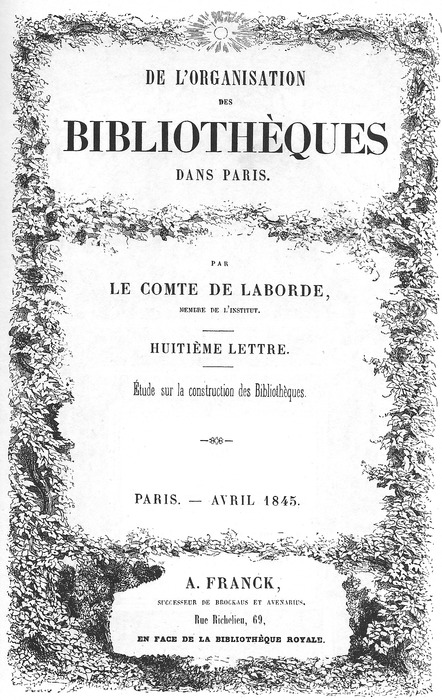
\includegraphics{img/wagner-2.jpg}
\caption*{Abb. 2: Frontispiz des achten Briefes von Léon de Laborde über
den Bau von Bibliotheken, 1845.}
\end{figure}

Die Verbreitung von Labordes Studie zum Bau und zur Organisation von
öffentlichen Bibliotheken über die \emph{Revue générale de
l'architecture et des travaux publics} verfolgt vor allem den Zweck, die
Architekten auf ebenjene Bauaufgabe vorzubereiten. (Abb. 3) Es sollen
ihnen die notwendigen Informationen für einen im Sinne Labordes und
Dalys funktionalen Bibliotheksbau an die Hand gegeben werden, dessen
Raumprogramm sich nicht auf ein äußerlich bleibendes Zitat der antiken
Ordnungen beschränkt, sondern von den verschiedenen Aufgaben der
Bibliothek, gleichsam von innen her, entwickelt wird. An solchen hatte
Laborde im Anschluss an das in den 1820er Jahren bereits erreichte
bibliothekarische Selbstverständnis bestimmt; es sei hier nur an
Leopoldo della Santa und Christian Molbech erinnert:\footnote{Die
  Laborde selbst zitiert. Vgl. hierzu Leopoldo della Santa, \emph{Über
  den Bau und die Verwaltung einer öffentlichen Universalbibliothek},
  mit einem veranschaulichenden Plan, Faksimile der Originalausgabe von
  1816, übersetzt v. Egon Wiszniewski, Karl-Marx-Stadt 1984; sowie den
  an Leopoldo della Santa anschließenden Christian Molbech, \emph{Ueber
  Bibliothekswissenschaft oder Einrichtung und Verwaltung öffentlicher
  Bibliotheken} (dän. 1829), übersetzt v. Henning Ratjen, Leipzig 1833.}
erstens die sichere Aufbewahrung von Büchern, zweitens eine leichte und
schnelle Recherche und drittens eine ungestörte Lektüre. Jeder dieser
Aufgaben entspricht ein eigener räumlicher Bereich: der Aufbewahrung das
Depot oder, wie es in Zusammenhang mit der modernen Bibliothek heißt,
das Magazin, der Recherche die Theke des Bibliothekars und ihr
zugeordnet der Katalog, der Lektüre der Lesesaal. Die von Laborde
verfolgte räumliche Ausdifferenzierung kennzeichnet den Übergang von der
barocken Saalbibliothek, in deren Raum noch alle drei Funktionen sowie
wesentlich diejenige der Repräsentation zusammenfallen, zur modernen
Magazinbibliothek. Dieser Übergang vollzog sich vom späten 18.
Jahrhundert bis zur Mitte des 19. Jahrhunderts, und zwar weniger über
vereinzelte Bauten\footnote{Wenn auch in einigen Bibliotheksneubauten
  aus der ersten Hälfte des 19. Jahrhunderts bereits eine räumliche
  Trennung von Lesesaal und Bücherverwahrung vorgenommen wurde, dann
  bleiben gerade die für die Buchbestände vorgesehenen Räume
  konzeptionell der Saalbibliothek verbunden, insofern die Bücher nach
  wie vor in Büchergalerien entlang der Wände untergebracht wurden. Die
  in der zweiten Hälfte des 19. Jahrhunderts sich durchsetzende moderne
  Magazinbibliothek als raumökonomische Weiterentwicklung des
  sogenannten \emph{stall system} wurde offensichtlich lediglich
  vorweggenommen durch die Hofbibliothek in Karlsruhe, 1765, die über
  Laborde Einzug in die Geschichte der Bibliotheksarchitektur gehalten
  hat, sowie durch die konkreten, jedoch nicht umgesetzten
  Bibliotheksentwürfe von Johann Conradin Beyerbach für Frankfurt, 1817,
  und Karl Friedrich Schinkel für Berlin, 1835. Zum Bibliotheksbau des
  19. Jahrhunderts vgl. im Überblick Hanns Michael Crass,
  \emph{Bibliotheksbauten des 19. Jahrhunderts in Deutschland}, München
  1976; Jean Bleton, \enquote{Les bâtiments}, in: \emph{Histoire des
  bibliothèques françaises}, tome 3: \enquote{Les bibliothèques de la
  Révolution et du XIXe siècle, 1789-1914}, hg. v. Dominique Varry,
  Paris 1991, S. 182-237.} als über eine Reihe bibliothekarischer und
architekturtheoretischer Schriften, in denen das moderne
Bibliotheksgebäude vor allem als Idee zirkulierte. Es ließe sich hier
ebenso gut von einer Phase der Latenz sprechen, in der der
Bibliotheksbau alle nur erdenklichen Dispositionen angenommen hat, bevor
sich dann ab der Mitte des 19. Jahrhunderts mit allgemein einsetzender
Bautätigkeit bestimmte Grundrisslösungen, Gebäudeformen und Baustile
durchsetzen und normativ werden. Hierher gehören die von
bibliothekarischer Seite aus bevorzugten Lösungen eines länglichen
Baukörpers, oft im Stil der Neorenaissance oder des Neobarock
ausgeführt, mit den räumlich voneinander getrennten Funktionen: dem
Lesesaal, der bis in das 20. Jahrhundert hinein in der Regel das
räumliche Zentrum der Bibliothek bildet, den Katalog- und
Verwaltungsräumen sowie zusehends einem schmucklosen Magazin mit
Flachdecken und Doppelrepositorien.\footnote{Zum Anfang des 20.
  Jahrhunderts erreichten Stand der Bibliotheksarchitektur vgl. Georg
  Leyh, \enquote{Bibliothek}, in: \emph{Wasmuths Lexikon der Baukunst},
  Bd. 1, Berlin 1929, S. 521-527.}

\begin{figure}[htbp]
\centering
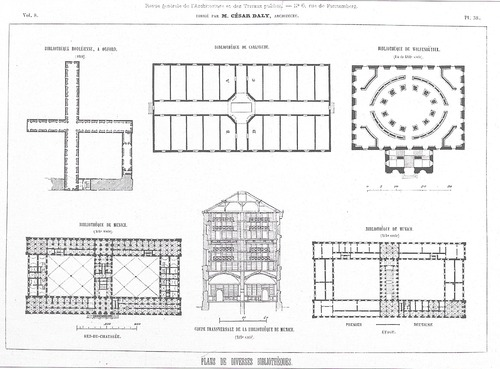
\includegraphics{img/wagner-3.jpg}
\caption*{Abb. 3: Tableau mit Grundrissen von Bibliotheksbauten in der
\emph{Revue générale d'architecture et des travaux publics}, tome 8,
1849-50.}
\end{figure}

Die scheinbar linear verlaufende Entwicklungsgeschichte der modernen
Bibliothek vom dysfunktionalen Schmuck- und Repräsentationsbau zum
zweckmäßig eingerichteten Funktionsbau hat das im späten 18. und frühen
19. Jahrhundert eröffnete Feld möglicher Bibliotheksarchitekturen in den
Hintergrund treten lassen. Indessen weist es ein auffallendes Spektrum
auf, und zwar nicht nur hinsichtlich der unterschiedlichen Genera und
Stile, in denen das Bibliotheksgebäude gedacht worden ist, sondern auch
der Anleihen an andere Gebäudetypen. In den zahlenmäßig kaum zu
überblickenden Entwürfen aus der ersten Hälfte des 19. Jahrhunderts
allein für die französische \emph{Bibliothèque royale} finden sich
Referenzen an Tempel, Theater, Kaserne, Fabrik und Gefängnis mit ihren
jeweils eigenen Raumordnungen, die immer auch Wissens- und
Körperordnungen sind. Das von bibliothekarischer Seite ausgesprochene
Verdikt gegenüber bestimmten Raumformen hat deren Verdrängung dabei
begünstigt, wenn sie auch nie ganz aus der Bibliotheksarchitektur
verschwunden sind. Ein Beispiel dafür geben Rundbauten und
Kuppellesesäle. Entgegen der durch Léon de Laborde oder Georg Leyh an
ihnen geübten Kritik\footnote{Vgl. Laborde, Étude sur la construction
  des bibliothèques, sowie Leyh, Bibliothek.} sind sie bis in die
Gegenwart hinein im Bibliotheksbau zu finden.\footnote{Vgl. hierzu im
  Überblick Ursula Bernhardt, \enquote{Die Kuppel über dem Quadrat: der
  neue Lesesaal in der Tradition bedeutender Kuppellesesäle}, in:
  \emph{Buch, Leser, Bibliothek: Festschrift der Badischen
  Landesbibliothek zum Neubau}, hg. v. Gerhard Römer, Karlsruhe 1992, S.
  93-113.}

Insgesamt macht die Bibliothekswissenschaft der Architektur die
Autorität über den Bibliotheksbau im 19. Jahrhundert streitig. Hatte die
Architekturtheorie\footnote{Zum Bibliotheksbau in der Architekturtheorie
  vgl. Regina Becker, \enquote{ordinatio et dispositio. Die Grundlagen
  einer Architektonik für die Bibliotheca publica}, in: Robert Felfe u.
  Kirsten Wagner (Hg.), \emph{Museum, Bibliothek, Stadtraum. Räumliche
  Wissensordnungen 1600-1900}, Berlin 2010, S. 89-108; dies.:
  \enquote{Theorie und Praxis -- zur Typologie in der
  Bibliotheksarchitektur des 17. und 18. Jahrhunderts}, in:
  Carsten-Peter Warncke (Hg.), \emph{Ikonographie der Bibliotheken},
  Wiesbaden 1992, S. 235-269.} an allgemeinen Bedingungen desselben bis
in das 19. Jahrhundert kaum mehr festgestellt, als dass das Gebäude
gegen Feuchtigkeit und Brandgefahr zu schützen sei, darüber hinaus den
natürlichen Lichteinfall zu berücksichtigen und diesen über die
Ausrichtung der Räume und ihre Fensteröffnungen zu verstärken
habe,\footnote{Daraus resultierten im Entwurf Büchersammlungen, die sich
  im ersten Stockwerk von Gebäuden befanden, Beamtenwohnungen, die aus
  dem eigentlichen Bibliotheksgebäude herausgelöst wurden -- wie
  überhaupt die Forderung nach einem frei stehenden Gebäude --, sowie
  schließlich an den beiden Längsseiten der Büchersäle vorhandene, höher
  gelegene Fensterreihen bis hin zu Fensteröffnungen in den Decken für
  entsprechendes Oberlicht.} dann wurde dies aus der bibliothekarischen
Praxis im 19. Jahrhundert um die voneinander getrennten Funktionsabläufe
in der Bibliothek und ein daraus abgeleitetes Raumprogramm erweitert.
Schon Laborde weiß zwischen solchen Bauten zu unterscheiden, bei denen
für Planung und Entwurf ausschließlich ein Architekt verantwortlich
gezeichnet hat -- Bauten, die seiner Kritik bezeichnender Weise nicht
standhalten --, und solchen, bei denen diese Aufgaben wesentlich vom
Bibliothekar beeinflusst worden sind. Während Leyh am Ende der
Entwicklung der modernen Magazinbibliothek den Architekten nur mehr als
Künstler und nur noch dort tätig werden lässt, wo es über die allgemeine
Disposition des Gebäudes hinaus um die \enquote{Parerga} von
Büchersammlungen geht: \enquote{{[}\ldots{}{]} die Gestaltung der
Fassade, der Eingangshalle, des Treppenhauses, der Lesesäle
{[}\ldots{}{]}}.\footnote{Leyh, Bibliothek, S. 522.}

Die Diskussion um die moderne Bibliotheksarchitektur verläuft
entsprechend an zwei seit dem späten 18. Jahrhundert gezogenen Grenzen:
zwischen Architekt und Ingenieur einerseits, zwischen Architekt und
Bibliothekar andererseits. Kennzeichen dieser Diskussion ist, dass sie
öffentlich über das Medium ausgetragen wird, das von sich beansprucht,
mit der Dynamisierung und Ausdifferenzierung des Wissens in der Moderne
Schritt halten zu können: die Presse, und hier im Besonderen die
Architekturpresse. Zum Konzept der \emph{Revue générale de
l'architecture et des travaux publics} als einer der wichtigsten
Architekturzeitschriften des 19. Jahrhunderts führt César Daly aus, dass
sie gegenüber dem statischen Buch, das sich angesichts des anwachsenden
Wissens bereits am Tag nach seinem Erscheinen als unvollständig erweise,
nicht nur die rasanten Fortschritte in den Wissenschaften und Künsten
besser abbilden könne, sondern auch der Kommunikation der neuesten
Erkenntnisse über die Fachgrenzen hinweg diene.\footnote{César Daly,
  \enquote{Introduction}, in: \emph{Revue générale de l'architecture et
  des travaux publics}, tome 1 (1840), S. 1-7, hier S. 4.} Nun nimmt der
Bibliotheksbau innerhalb der \emph{Revue générale de l'architecture et
des travaux publics} vielleicht nicht die wichtigste Rolle ein. In der
Zeitschrift herrschen neben praktisch konstruktiven Fragen
architekturhistorische Themen mit einem Fokus auf der mittelalterlichen
und der außereuropäischen Architektur vor. Hinzu kommen die neuen
Bauaufgaben im Wohnungs-, Schul-, Gesundheits- und Transportwesen.

Dennoch zeigt sich Dalys Periodikum als zentrales Forum in der
Auseinandersetzung um die \emph{Bibliothèque royale} und damit verbunden
den modernen Bibliotheksbau. Nicht nur kommen die konträren Lager,
Bestandserhalt und Umbau der \emph{Bibliothèque royale} im Palais
Mazarin versus Abriss und Neubau an einem anderen Standort, über die
Präsentation der jeweiligen Entwürfe zu Wort. Es werden, wie an Dalys
eingangs zitiertem Beitrag zu sehen ist, auch allgemeine Reflexionen
über die Bibliotheksarchitektur angestellt.\footnote{Wenn die von Marc
  Saboya ausgewertete Anzahl der in der \emph{Revue générale} \emph{de
  l'architecture et des travaux publics} vorgestellten
  Bibliotheksentwürfe nahelegt, dass es sich beim Bibliotheksbau um
  einen in der Zeitschrift vergleichsweise wenig berücksichtigten
  Gegenstand handelt, ist das ein Stück weit zu relativieren. Denn mit
  der Konzentration auf einzelne konkrete Entwürfe übersieht Saboya,
  dass über die verschiedenen Rubriken der Zeitschrift verteilt,
  besonders in den Miszellen, immer wieder an die laufende
  Bibliotheksdiskussion angeschlossen wird, etwa mit Berichten über
  aktuelle Planungen und behördliche Bekanntmachungen in Zusammenhang
  mit der \emph{Bibliothèque royale}. Hinzu kommt, dass Artikel wie der
  abgedruckte vierte Brief Labordes über den Palais Mazarin in
  unmittelbarem Zusammenhang mit der Bibliotheksfrage steht. Vgl. hierzu
  Marc Saboya, \emph{Presse et architecture au XIXe siècle. César Daly
  et la Revue générale de l'architecture et des travaux publics}, Paris
  1991, insbes. S. 272 f.} Für die Darstellung des Bibliotheksbaus in
der Architekturpresse gilt daher, was Marc Saboya generell für das neue
Medium der Architekturperiodika festgestellt hat: Jene zeichnen ein
direktes Bild der im 19. Jahrhundert geführten stilistisch-ästhetischen
Kontroversen und öffentlichen Meinungsbildung über bestimmte
Bauaufgaben, so auch über die moderne Bibliothek. Auf diese Weise
vermitteln die Architekturperiodika zugleich den \enquote{caractère
collectif de l'activité architecturale}.\footnote{Ebd., S. 50.} Dies
gilt in besonderem Maße für den Bibliotheksbau, zu dem sich im frühen
19. Jahrhundert neben Architekten und Bibliothekaren auch
Altertumsforscher, Künstler, Industrielle und Bankiers, private Sammler
und Philanthropen äußerten. Sie waren nicht nur die Adressaten der
\emph{Revue générale de l'architecture et des travaux
publics,}\footnote{Bereits in der ersten Ausgabe der \emph{Revue
  générale de l'architecture et des travaux publics} wird von Daly
  benannt, an wen sich die Zeitschrift gleichermaßen richtet:
  \enquote{{[}\ldots{}{]} à la fois aux architects, aux ingénieurs, aux
  archéologues, aux industriels, aux propriétaires, et enfin aux
  governments {[}\ldots{}{]}.} Daly, Introduction, S. 4.} sie fanden
dort auch ein Sprachrohr, über das ihre Entwürfe und architektonischen
Ideen verbreitet wurden.

Unter diesen interessieren im Folgenden drei Entwürfe, die im zweiten
Jahrgang der \emph{Revue générale de l'architecture et des travaux
publics} durch einen offensichtlich anonym bleiben wollenden
Bibliophilen (sic!) vorgestellt werden. Es handelt sich hierbei um die
Entwürfe von Jean Chevret (1747-1820), einem \enquote{einfachen
Angestellten der königlichen Bibliothek}\footnote{Anonymus, \enquote{La
  Bibliothèque royale}, in: \emph{Revue générale de l'architecture et
  des travaux publics}, 3 (1842), S. 307-308, hier S. 308.},
Antoine-François Mauduit (1775-1854), seines Zeichens Architekt und
ehemaliger Sekretär und Bibliothekar der \emph{Académie de France} in
Rom, sowie Benjamin Delessert (1773- 1847), Bankier und in
Wissenschaftskreisen weithin angesehener Besitzer einer Pflanzen- und
Muschelsammlung nebst dazugehörender naturkundlicher Bibliothek. Alle
drei teilen die Konzeption einer Bibliotheksrotunde mit zentralem
Lesesaal. Geht es dem bibliophilen Rezensenten mit der Darstellung
dieser Entwürfe vor allem um die Klärung des Urheberrechts an der
zirkulären und radialen Raumordnung von Büchersammlungen, dann sollen
hier die verschiedenen Wissens- und Körperordnungen im Vordergrund
stehen, die sich im Übergang von der Saal- zur Magazinbibliothek in den
Rundbau einschreiben und überlagern: zum einen die Verräumlichung eines
enzyklopädischen, universalen Wissens und zum anderen die panoptische
Regulierung von Körperbewegungen, von Buchkörpern und
Nutzerkörpern\footnote{Zu diesem Aspekt der Bewegung in Bibliotheken
  vgl. exemplarisch Ulrich Johannes Schneider, \enquote{Bücher und
  Bewegung in der Bibliothek von Herzog August}, in: Frank Büttner,
  Markus Friedrich u. Helmut Zedelmaier (Hg.), \emph{Sammeln, Ordnen,
  Veranschaulichen. Zur Wissenskompilatorik in der Frühen Neuzeit},
  Münster 2003, S. 111-127.}, im Raum. Eine Verbindung zwischen diesen
unterschiedlichen architektonischen Bibliotheksideen besteht dort, wo
das räumliche Zentrum mit einem allsehenden und allwissenden Auge
besetzt zu sein scheint.

\subsubsection{\texorpdfstring{Entwürfe der modernen Bibliothek im
historischen Kontext der \emph{Bibliothèque
royale}}{Entwürfe der modernen Bibliothek im historischen Kontext der Bibliothèque royale}}\label{entwuxfcrfe-der-modernen-bibliothek-im-historischen-kontext-der-bibliothuxe8que-royale}

Die Entwürfe für einen Bibliotheksneubau von Chevret, Mauduit und
Delessert teilen nicht nur den Rundbau, sie beziehen sich allesamt auf
die \emph{Bibliothèque royale} in Paris, deren Anfänge bis auf die
Handschriftensammlungen Karls V. in das 14. Jahrhundert
zurückreichen.\footnote{Zur Geschichte der \emph{Bibliothèque royale}
  vgl. im Überblick Françoise Bléchet, \enquote{La Bibliothèque royale
  du XVIe siècle à 1789}, in: Myriam Bacha u. Christian Hottin (Hg.),
  \emph{Les bibliothèques Parisiennes. Architecture et décor}, Paris
  2003, S. 45-50.} Nach verschiedenen Standorten außerhalb und innerhalb
von Paris zog die königliche Bibliothek, die mittlerweile mehr als
105.000 Handschriften und 40.000 gedruckte Werke umfasste,\footnote{Ebd.,
  S. 47.} in den 1720er Jahren in die Räumlichkeiten des Palais Mazarin
ein. In diesem Zuge erfolgten einige Umbaumaßnahmen des
Gebäudeensembles. (Abb. 4) Noch im 18. Jahrhundert zeigte sich indessen,
dass der heterogene Gebäudekomplex trotz der neu eingerichteten Galerien
und Erweiterungen für die stetig anwachsenden Bestände nicht mehr
ausreichte. Ein öffentlicher Lesesaal der seit 1692 allgemein
zugänglichen Bibliothek fehlte ebenfalls. Zudem wurden an den
historischen Gebäuden des Palais Mazarin erste Schäden festgestellt, und
von Seiten benachbarter Gebäude drohte Brandgefahr. Entsprechend setzten
bereits in der zweiten Hälfte des 18. Jahrhunderts Planungen für eine
Erweiterung oder Auslagerung der königlichen Bibliothek ein.

\begin{figure}[htbp]
\centering
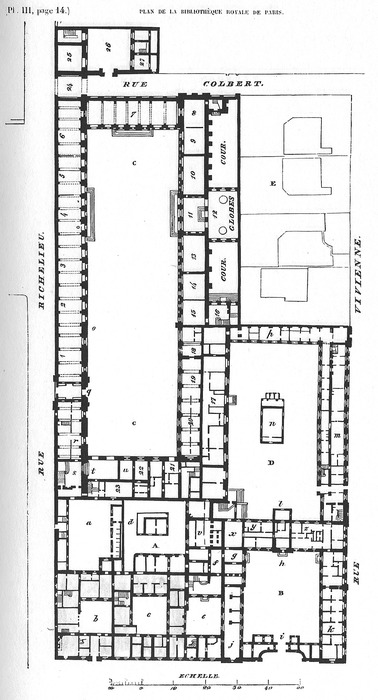
\includegraphics{img/wagner-4.jpg}
\caption*{Abb. 4: Grundriss der \emph{Bibliothèque royale} im Palais
Mazarin nach León de Laborde, 1845.}
\end{figure}

Unter diesen Planungen befinden sich auch mehrere Entwürfe von
Étienne-Louis Boullée, die sich jeweils auf einen anderen Standort in
Paris beziehen.\footnote{Die beiden anderen Entwürfe richteten sich auf
  das Gelände des Kapuzinerordens sowie einen Standort in der Nähe des
  Palais Mazarin. Während der erste einen kreuzförmigen Grundriss mit
  einer halbkreisförmigen, von Säulenkolonnaden gerahmten Vorhalle
  (Apollotempel) aufweist, organisiert sich der zweite um einen
  zentralen Hof. Zu Boullées Bibliotheksentwürfen vgl. Étienne-Louis
  Boullée, \emph{Architektur. Abhandlung über Kunst}, hg. v. Beat Wyss,
  eingeführt u. kommentiert v. Adolf Max Vogt, übersetzt v. Hanna Böck,
  Zürich u. München 1987, S. 117-123; Helen Rosenau, \emph{Boullée's
  Treatise on Architecture}, London 1953, S. 18 f.; Jean-Marie Pérouse
  de Montclos, \emph{Étienne-Louis Boullée (1728-1799), de
  l'architecture classique à l'architecture revolutionnaire}, Paris
  1969, S. 125-127, 165-167; Adolf Max Vogt, \enquote{Boullée sucht
  «kosmische Größe für seine Bibliothek»}, in: Susanne Bieri u. Walther
  Fuchs (Hg.), \emph{Bibliotheken bauen. Tradition und Vision}, Basel
  u.a. 2001, S. 215-226.} (Abb. 5) Der bekannteste unter ihnen sah eine
Überbauung des Hofes zwischen der Galerie Mazarine und dem westlichen
Flügel des Hôtel Nevers mit einem kassettierten Gewölbebogen vor, der
den gesamten Hof über eine Fläche von rund 2.508 qm\textsuperscript{2}
überspannt. An den Längsseiten des Hofes, unterhalb der Säulenreihen,
durchlaufen jeweils vier terrassenförmig angelegte Bücherwände mit einem
Fassungsvermögen von mehr als 300.000 Bänden\footnote{Für diese Anzahl
  allein an gedruckten Büchern plante Boullée seine Bibliothek.} den
gesamten Raum. Im Scheitelpunkt des Tonnengewölbes ist ein Oberlicht
ausgespart. Die Zeichnung unterstreicht die Monumentalität des
Entwurfes, indem die zentralperspektivische Raumkonstruktion nicht nur
einen durch die Säulenreihen massierten Tiefensog entfaltet, sondern mit
dem niedrig gelegenen Fluchtpunkt auch die Höhendimension des Raumes
betont. Gegenüber der regelmäßigen Ordnung des Raumes weisen die Bücher
eine dynamische Ordnung auf: Ins Rutschen gekommene Buchreihen oder
aufeinander gestapelte Bände zeigen die Bücher in Bewegung an. Auch die
antikisiert dargestellten Nutzer der Bibliothek, die sich aufgrund der
Größenverhältnisse in diesem ausgedehnten, kosmischen Raum des Wissens
zu verlieren scheinen, sind nicht einfach in stiller Lektüre erstarrt.
Sie führen Zeigegesten des geometrischen und literarischen Beweises aus,
betrachten Globen, disputieren, ziehen Bücher aus den Regalen. Wenn
Boullée selbst als Vorbild für seine Bibliotheksentwürfe Raffaels Fresko
\emph{Die Schule von Athen} in den Vatikanischen Stanzen aus den Jahren
1509-1511 angegeben hat, dann umfasst die Adaptation mehrere Ebenen:
erstens das kassettierte Gewölbe sowie den Triumphbogen als
architektonische Zitate,\footnote{Dabei weist Boullées
  Bibliotheksentwurf auf dem Gelände des Kapuzinerordens mit seinem
  kreuzförmigen Grundriss und dem Kuppelsaal im Zentrum eine noch
  größere Nähe zu der ihrerseits an antiken Vorbildern orientierten
  Bildarchitektur Raffaels auf.} zweitens die Figurenanordnung -- auf
der rechten Bildhälfte im geometrischen Beweis, auf der linken Hälfte in
aufgeschlagene Bücher bzw. Kodizes vertiefte Figuren --, drittens die
Konzeption der Bibliothek als eine ebenso kommemorativ wie edukativ
angelegte Versammlung sämtlicher Geistesgrößen und der durch sie
verkörperten Wissenschaften und Erkenntnisse in einem Raum.\footnote{Vgl.
  Boullée, Architektur, S. 117.}

\begin{figure}[htbp]
\centering
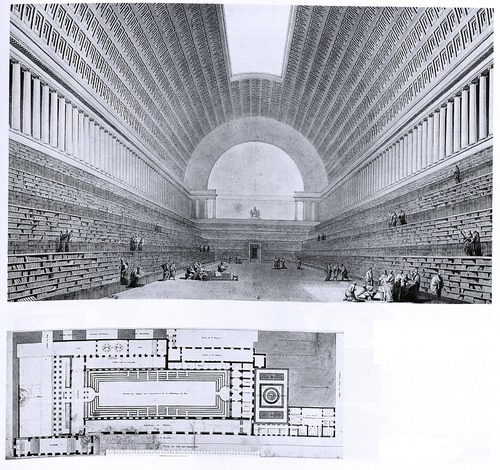
\includegraphics{img/wagner-5.jpg}
\caption*{Abb. 5: Entwurf für die \emph{Bibliothèque royale} von
Étienne-Louis Boullée, 1785.}
\end{figure}

Boullée hat für den hier gezeigten Entwurf die Bilder einer
\enquote{riesigen, von oben beleuchteten Basilika} und eines
\enquote{nur aus Büchern bestehende{[}n{]}
Amphitheater{[}s{]}}\footnote{Ebd., S. 120, 122.} gefunden. Kommen in
ihm noch einmal Lesesaal und Buchaufstellung im Sinne der barocken
Saalbibliothek mit ihrem auf die gleichermaßen ästhetische und
repräsentative Wirkung der Bücherwände zielenden Programm zusammen,
bedenkt Boullée bereits eine Ausdifferenzierung der Bestände, insofern
in den angrenzenden Räumen des Palais Mazarin, zum Teil der bestehenden
Sammlungsaufteilung folgend, die Manuskripte, Stiche, Münzen und
zusammen mit den Coronelli Globen die Geographica untergebracht
werden.\footnote{Zur Raum- und Sammlungsaufteilung der
  \emph{Bibliothèque royale} im Palais Mazarin vgl. Léon de Laborde,
  Étude sur la construction des bibliothèques, S. 14-16.}
Bibliotheksökonomische Überlegungen zur schnellen Buchbeschaffung über
den direkten Zugriff und die unmittelbare Buchausgabe am Regal durch die
Bibliothekare sowie die gleichzeitig gegebene Möglichkeit der
Überwachung der Leser weisen ebenfalls schon über die Saalbibliothek
hinaus. Boullée führt in diesem Zusammenhang die antike Bibliothek Roms
als Vorbild an. Ihre Vorzüge hätten darin gelegen, dass die
\enquote{Galerien von einem gemeinsamen Zentrum ausgehen, so dass man
von dort alle in der Bibliothek befindlichen Personen sehen
kann}\footnote{Boullée, Architektur, S. 119. Nach Rosenau soll sich
  Boullée hier auf einen (missverstandenen) Passus aus Plinius'
  Naturgeschichte, Buch 7.xxx, beziehen, in dem Plinius über die erste
  von Gaius Asinius Pollio im Atrium Libertatis gegründete öffentliche
  Bibliothek Roms berichtet. Die von ihren Räumlichkeiten bis heute
  nicht eindeutig rekonstruierte Bibliothek wurde durch Beutezüge des
  Pollio ermöglicht, und in ihr sollen Bildnisse der bedeutendsten
  Schriftsteller der Antike, darunter eines von Marcus Terentius Varro,
  des einzigen lebenden unter den so geweihten Autoren, aufgestellt
  gewesen sein. Vgl. hierzu Rosenau, Boullées Treatrise, S. 114.}.
Ebendieser Überwachungstopos wird sich über Durands radialen
Bibliotheksentwurf fortsetzen und in Delesserts panoptischer Form der
Bibliothek gleichsam zu sich selbst kommen.

Die Entwürfe Boullées umspannen im Wesentlichen das Spektrum, zwischen
dessen Polen sich die Diskussion um die \emph{Bibliothèque royale} in
den Jahren 1750 bis 1850 bewegte: Zwischen einem Bestandserhalt im
Palais Mazarin mit entsprechenden Eingriffen in die vorhandene
Bausubstanz und einem Neubau, für den alle nur erdenklichen Formen und
Standorte links und rechts der Seine in Betracht gezogen
wurden.\footnote{Zu den verschiedenen in Erwägung gezogenen Standorten
  vgl. ausführlich den kritischen Beitrag Léon de Labordes, La
  Bibliothèque Royale occupe le centre topographique.} Als Alternative
kam mehrfach eine Überführung der Bibliothek und ihre Zusammenlegung mit
anderen Sammlungsbeständen der Künste und Wissenschaften im Louvre auf.
Am Ende wurde die Diskussion mit dem Entwurf des
\enquote{Architekten-Konstrukteurs}\footnote{Wie Sigfried Giedion
  Labrouste als den Architekten des 19. Jahrhunderts charakterisiert,
  der zum \enquote{erstenmal Ingenieur und Architekt in einer Person
  Gestalt} hat werden lassen. Vgl. Sigfried Giedion, \emph{Bauen in
  Frankreich. Bauen in Eisen. Bauen in Eisenbeton} (1928), neu hg. u.
  mit einem Nachwort versehen v. Sokratis Georgiadis, Berlin 2000, S.
  14.} Henri Labrouste, seit 1854 Nachfolger Louis Viscontis im Amt des
Architekten der königlichen Bibliothek, zugunsten des Bestandserhalts
und -umbaus entschieden. Nahezu an der Stelle, an der Boullée seinen
Büchertempel geplant hatte, entstand in den Jahren 1861-1869 basierend
auf einer Eisenkonstruktion ein von neun Kuppeln überspannter Lesesaal
mit angeschlossenem Magazin.\footnote{Zum Bibliotheksentwurf von Henri
  Labrouste vgl. Julien Cain, Roger-Amand Weigert u. Jean Valley-Radot,
  \emph{Labrouste. Architecte de la Bibliothèque Nationale de 1854 à
  1875}, Ausstellungskat., hg. v. der Bibliothèque nationale, Paris
  1953.} (Abb. 6) In den gut sieben Jahrzehnten, die zwischen Boullées
Entwürfen und der Erweiterung des Palais Mazarin durch Henri Labrouste
liegen, tauchte auf dem Papier eine Vielzahl weiterer Bibliotheksbauten
auf. Zum einen resultierten sie aus Wettbewerben, die zum täglichen
Lehrbetrieb der \emph{École des beaux-arts} gehörten. Allein der
\emph{Grand Prix de Rome} hatte 1814 eine mit einem Museum verbundene
Bibliothek und 1828 eine öffentliche Bibliothek zum
Gegenstand.\footnote{Vgl. hierzu Jean-Michel Leniaud, \enquote{Le
  programme d'une bibliothèque au XIXe siècle}, in: ders. (Hg.),
  \emph{Des palais pour les livres. Labrouste, Sainte-Geneviève et les
  bibliothèques}, Paris 2002, S. 11-23.} Zum anderen fühlten sich
inzwischen auch \enquote{Laien} wie Benjamin Delessert berufen, sich mit
eigenen Entwürfen in die öffentlich geführte Bibliotheksdiskussion
einzuschalten, die im ersten Drittel des 19. Jahrhunderts an
Dringlichkeit zugenommen hatte. Durch die Säkularisation und die
Französische Revolution waren zahlreiche Kloster- und Privatbibliotheken
beschlagnahmt beziehungsweise aufgelöst worden. Die in Umlauf gebrachten
und zum Teil der \emph{Bibliothèque royale} zugeführten Handschriften
und -buchbestände brachten das räumliche Fassungsvermögen der Bibliothek
mit im Jahr 1835 gezählten 750.000 Büchern und über 100.000
Handschriften endgültig an seine Grenzen. Auch der Nutzerkreis von
Bibliotheken erweiterte sich. Symptomatisch bezieht Léon de Laborde in
seine Standortanalyse der verschiedenen Pariser Bibliotheken die
\enquote{ouvriers littéraires} als neue Adressaten ein, die in den
Lesesälen ihr Tagesgeschäft verrichteten.\footnote{Laborde, La
  Bibliothèque Royale occupe le centre topographique. Im achten Brief,
  Étude sur la construction des bibliothèques, S. 47, unterscheidet
  Laborde zudem zwischen dem in der Bibliothek arbeitenden
  Wissenschaftler (\enquote{travailleur}) und dem nur zur Besichtigung
  ihrer Sammlungsbestände sie Aufsuchenden (\enquote{visiteur}). Die
  Domäne des ersten ist der Lesesaal, die des zweiten das von Laborde in
  seinen Bibliotheksentwürfen vorgesehene, der eigentlichen Bibliothek
  vorgelagerte \emph{Musée}, das neben Statuen eine historische
  Ausstellung der grafischen Künste sowie an Abteilungen die Münzen,
  Antiken und Rara enthält.} Die öffentliche Bibliothek erscheint nicht
mehr wie bei Boullée als nationaler Geistes- und Wissenstempel, sondern
gemäß dem Eingangszitat César Dalys als Arbeits-, Bildungs- und
Erziehungsinstrument für breitere Schichten der Gesellschaft. In
letzterer Funktion wurde sie zugleich zu einem Gegenstand der
philanthropischen Bewegung des 19. Jahrhunderts.

\begin{figure}[htbp]
\centering
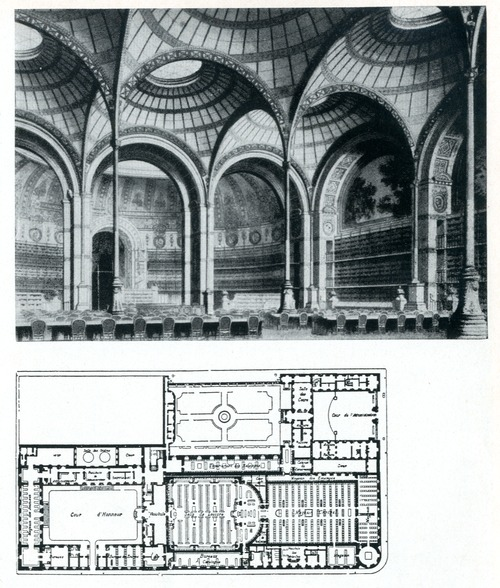
\includegraphics{img/wagner-6.jpg}
\caption*{Abb. 6: Erweiterungsbau bzw. Lesesaal und Magazin für die
\emph{Bibliothèque royale} von Henri Labrouste, 1861-1869.}
\end{figure}

\subsubsection{Entwürfe der modernen Bibliothek: zwischen Kolosseum,
Pantheon und
Panopticon}\label{entwuxfcrfe-der-modernen-bibliothek-zwischen-kolosseum-pantheon-und-panopticon}

Vor diesem Hintergrund sind auch die drei 1842 in der \emph{Revue
générale de l'architecture et des travaux publics} vorgestellten
Entwürfe von Chevret, Delessert und Mauduit zu sehen, auf die jetzt
zurückzukommen ist. Alle teilen den Rundbau beziehungsweise eine
ellipsenförmige Rotunde mit zirkulärer oder aber radialer
Grundrissorganisation. Während Mauduit seinen Entwurf explizit auf
Bauten der römischen Antike zurückführt, ruft Delessert mit seinem
Konzept einer \enquote{forme panoptique}\footnote{Benjamin Delessert,
  \emph{Mémoire sur la Bibliothèque royale, ou l'on indique les mesures
  à prendre pour la transférer dans un bâtiment circulaire, d'une forme
  nouvelle, qui serait construit au centre de la Place du Carrousel},
  Paris 1835, S. 4.} stillschweigend das von Jeremy Bentham im Ausgang
des 18. Jahrhunderts in mehreren Briefen vorgestellte
Panopticon,\footnote{Jeremy Bentham, \emph{Panopticon; or the
  inspection-house, containing the idea of a new principle of
  construction applicable to any sort of establishment, in which persons
  of any description are to be kept under inspection; and in particular
  to penitentiary-houses, prisons, houses of industry, work-houses,
  poor-houses, lazarettos, manufactories, hospitals, mad-houses, and
  schools} (1787), Dublin 1791.} eine Gefängnisarchitektur, auf. Chevret
hingegen sucht noch einmal Anschluss an die verräumlichten
Wissensordnungen der frühen Neuzeit. Innerhalb der
Bibliotheksarchitektur ist die Rotunde keineswegs neu.\footnote{Eine
  tabellarische Übersicht über die Bibliotheksrotunden des 17. und 18.
  Jahrhunderts gibt Petra Hauke, \emph{Domus Sapientiae. Ein Beitrag zur
  Ikonologie der Bibliotheksraumgestaltung des 17./18. Jahrhunderts
  unter besonderer Berücksichtigung des Klosters St.~Mang, Füssen}, Bad
  Honnef 2007, S. 183.} Die \emph{Bibliotheca Augusta} in Wolfenbüttel,
1706 bis 1710 nach Plänen von Hermann Korb realisiert, gilt innerhalb
der Bibliotheksarchitektur als erster frei stehender Zentralbau mit
einer innen liegenden ellipsenförmigen Rotunde. Zu den Vorbildern zählen
das Pantheon und die Villa Rotonda Andrea Palladios.\footnote{Vgl.
  Markus Eisen, \enquote{Zur architektonischen Typologie von
  Bibliotheken}, in: Winfried Nerdinger (Hg.), \emph{Die Weisheit baut
  sich ein Haus. Architektur und Geschichte von Bibliotheken}, München
  u.a. 2011, S. 261-306.} Als Ellipse ausgeführt wurde auch die
Bibliothek des Klosters St.~Mang in Füssen.\footnote{Vgl. Hauke, Domus
  Sapientiae, darin auch Ausführungen zur Ellipse in der
  Architekturtheorie und im Bibliotheksbau, S. 180-181. Über den Hinweis
  auf Kepler liegt ein Ausblick auf die Kulturwissenschaftliche
  Bibliothek Warburg mit ihrem ellipsoiden Lesesaal nahe.} Bei ihr
handelt es sich jedoch um kein autonomes Bibliotheksgebäude, vielmehr
ist sie Teil der von 1701 bis 1718 auf einem romanischen Vorgängerbau
errichteten Klosteranlage. Bereits in den 1670er Jahren hatte
Christopher Wren einen ebenfalls durch die Villa Rotonda inspirierten
Bibliotheksentwurf für das Trinity College in Cambridge
vorgelegt.\footnote{Vgl. hierzu Howard Colvin, der die Rotunde Wrens auf
  Palladio zurückführt: \enquote{For a circular library there was no
  precedent, ancient or modern, but plans of a centralised character
  made a strong appeal to Wren, as they had done to so many European
  architects from the Renaissance onwards. What Wren envisaged for
  Trinity would have looked externally somewhat like Palladio's Villa
  Rotonda near Vicenza, but with only one portico, and that an attached,
  not a free-standing, one.} Howard Colvin, \enquote{The building}, in:
  David McKitterick (Hg.), \emph{The making of the Wren Library, Trinity
  College, Cambridge}, Cambridge 1995, S. 28-49, hier S. 32.} (Abb. 7)
Die Bibliotheksrotunde zeigt sich bei Wren von einem kubischen Baukörper
ummantelt, über den sich eine von einer Laterne bekrönte Kuppel erhebt.
Weitere Bibliotheksrotunden sind mit den Entwürfen der Wren-Schüler
Nicholas Hawksmoor und James Gibbs für die Radcliffe Library in Oxford
gegeben, deren Errichtung in den Jahren 1737-1749 schließlich Gibbs
oblag.\footnote{Vgl. Ralph Dutton, \emph{The Age of Wren}, London u.a.
  1951. Das Bibliotheksgebäude ist dokumentiert über James Gibbs,
  \emph{Bibliotheca radcliviana: or, a short description of the
  Radcliffe library at Oxford}, London 1747.} Dabei wurde die Rotunde
aus jeglicher Ummantelung herausgeschält. Die genannten Zentral- und
Rundbauten verbindet die zirkuläre Aufstellung der Bücher an den
umlaufenden Wänden im Inneren der Rotunden. Jean-Nicolas-Louis Durand
wandelte diese Disposition insofern ab, als sein in dem \emph{Précis des
leçons d'architecture} veröffentlichter Entwurf eines Zentralbaus von
acht Büchergalerien ausgeht, die strahlen- oder sternförmig von einem
Kuppelsaal wegführen und in einen umlaufenden Gebäudering
münden.\footnote{An wenn auch in Bezug auf die Gebäudeart Bibliothek
  \enquote{unvollständigen} Vorbildern benennt Durand den Rundbau der
  Radcliviana sowie den kreuzförmigen Grundriss mit überkuppelter
  Vierung der Bibliothek \emph{Sainte-Geneviève}. Jean-Nicolas-Louis
  Durand, \emph{Précis des leçons d'architecture données à l'école
  polytechnique}, Paris 1805, S. 55.} (Abb. 8) Durand begründet diese
Disposition, bei der die Bibliothekare im Kuppelsaal untergebracht sind,
um von dort aus die Bücher- und Lesesäle in den Galerien einsehen zu
können, mit einer durch sie ermöglichten Ordnung und Überwachung
innerhalb der Bibliothek.

\begin{figure}[htbp]
\centering
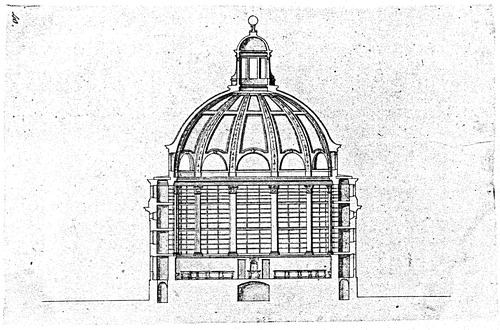
\includegraphics{img/wagner-7.jpg}
\caption*{Abb. 7: Entwurf einer Bibliotheksrotunde für das Trinity
College in Cambridge von Christopher Wren, 1670er Jahre.}
\end{figure}

\begin{figure}[htbp]
\centering
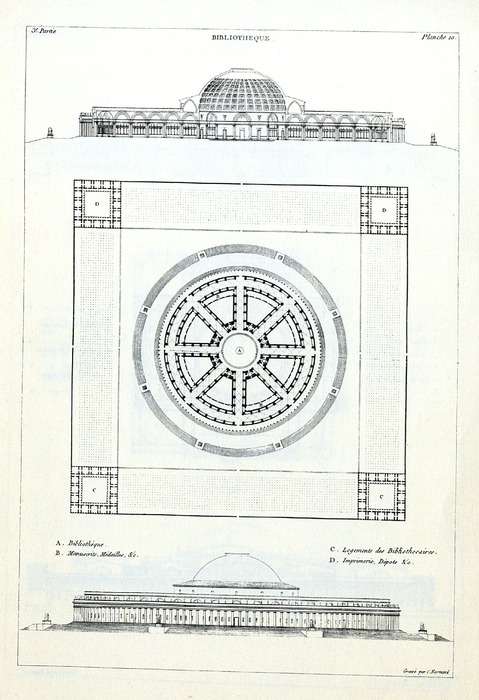
\includegraphics{img/wagner-8.jpg}
\caption*{Abb. 8: Radialer Bibliotheksentwurf von Jean-Nicolas-Louis
Durand, 1805}
\end{figure}

Auffällig an den Entwürfen von Chevret, Delessert und Mauduit ist, dass
sie wie Mauduit zwar an solche Architekturtopoi wie das Pantheon
anschließen, jedoch auf die zu ihrer Zeit bereits entworfenen und
ausgeführten Bibliotheksrotunden keinerlei Bezug nehmen. Auch der
bibliophile Rezensent der \emph{Revue générale de l'architecture et des
travaux publics}, der in Chevrets Entwurf das Vorbild für Delessert und
Mauduit gefunden haben will, stellt weder eine Verbindung zu anderen
Bibliotheksbauten noch zu anderen Gebäudetypen her. Damit entgeht ihm --
und das gilt fast ausnahmslos auch für die spätere Historiographie der
Bibliotheksarchitektur --, dass sich mit der Form des Rundbaus im
Übergang zur Moderne verschiedene Bedeutungen verbinden. Dies soll
abschließend an den Bibliotheksentwürfen Jean Chevrets, Antoine-François
Mauduits und Benjamin Delesserts nachvollzogen werden.

\subsubsection{Eine zentralistische Bildungsidee: der Bibliotheksentwurf
Jean
Chevrets}\label{eine-zentralistische-bildungsidee-der-bibliotheksentwurf-jean-chevrets}

Als Quelle des Bibliotheksentwurfs von Chevret führt der bibliophile
Rezensent dessen 1792 erschienene Schrift \emph{De l'éducation dans la
République}\footnote{Jean Chevret, \emph{De l'éducation dans la
  République, et de ses moyens de prospérité et de gloire, ou Suite du
  principe universel d'éducation}, Paris 1792.} an. Seit 1765 in der
\emph{Bibliothèque royale} tätig, trat Chevret in den ersten Jahren der
Französischen Revolution mit einer Reihe kleinerer Schriften an die
Öffentlichkeit, die zur Gattung der moralischen und politischen
Katechismen zu rechnen ist. Jene waren der Form nach am religiösen
Katechismus, einer belehrenden Unterweisung in christliche
Glaubensgrundsätze, orientiert, wurden im Rahmen der Revolution jedoch
mit republikanischen Gesellschaftsmaximen als weltlichen Inhalten
gefüllt und unter das Volk gebracht. Chevret bediente diese Gattung mit
gleichermaßen religiöser und politischer Emphase, was so sicherlich nur
in den Anfangsjahren der Revolution möglich gewesen ist. In einem kurzen
Nachruf über Chevret heißt es entsprechend, dass er die \enquote{Ursache
der Freiheit {[}das heißt die Revolution, Anm. K.W.{]} mit einem
Enthusiasmus umarmt hatte, der ihn oft zum Deklamieren verleitet, der
ihn aber niemals die religiösen und christlichen Prinzipien vergessen
ließ, von denen er sich überall lebhaft durchdrungen zeigt}.\footnote{Alphonse
  Mahul, \emph{Annuaire nécrologique, ou Supplément annuel et
  continuation de toutes les biographies ou dictionnaires historiques;
  contenant la vie de tous les hommes célèbres par leur écrits, leurs
  vertus ou leur crimes, morts dans le cours de chaque année; à
  commencer de 1820}, Paris 1821.} Dies gilt auch für seine Schrift von
1792, in der er die Erziehung der Jugend als notwendige Voraussetzung
für das republikanische Staatswesen herausstellt. Denn allein durch
Erziehung kann der nunmehr im Wollen und Handeln freie Bürger angeleitet
werden, das zu tun, was nicht nur in seinem Sinne, sondern auch im Sinne
des Gemeinwohls und gemäß den Naturgesetzen der Schöpfung das Richtige
und Wahre ist.

Dieser Erziehungsauftrag wird durch eine Bibliothek, die
\emph{Bibliothèque de la République}, verkörpert, die Chevret in
Korrespondenz zu einem Mausoleum entwickelt. Wie das Mausoleum die
sterblichen Überreste der Vorfahren aufnimmt und Ort des Gedenkens an
sie ist, so nimmt die Bibliothek zu kommemorativen und edukativen
Zwecken die Erzeugnisse des menschlichen Geistes auf.\footnote{Zur
  Verbindung von Mausoleum bzw. Grabmonument und Bibliothek schon bei
  Boullée vgl. Vogt, Boullée sucht «kosmische Größe für seine
  Bibliothek».} Die Disposition der \enquote{à la gloire de l'esprit
humain et du génie françois, la patrie reconnaissante}\footnote{Chevret,
  De l'éducation dans la République, S. 12.} geweihten Bibliothek leitet
Chevret dabei aus seiner bibliothekarischen Tätigkeit ab: \enquote{Nach
der Erfahrung, die wir seit 27 Jahren im öffentlichen Betrieb und in den
Arbeiten haben, zu denen wir besonders beauftragt worden sind während
der großen zu bewirkenden Bewegungen in der Bibliothèque Nationale,
scheint uns die zweckmäßigste Anordnung diejenige eines Sterns sein zu
müssen, überragt in seiner Mitte von einer Kuppel oder einem Kuppeldach;
das wäre die vorteilhafteste, die dem Auge am angenehmsten und, für die
Flinkheit und Schnelligkeit des öffentlichen Betriebes, die bequemste
Anordnung. Die fünf großen bibliographischen Unterteilungen geben
natürlicher Weise die Zahl der Galerien vor, die diesen Stern bildeten,
welche, alle vereint durch eine kreisförmige Galerie, ein Ganzes
formten, das fähig wäre, die gedruckten Bücher, die Handschriften, die
Stiche, die Münzen, und die anderen zur Bibliothek gehörenden
Sonderbestände zu enthalten, die sich alle, wenn auch voneinander
separiert, der Öffentlichkeit vermittelten.}\footnote{Ebd.}

In ebenjener Textpassage findet der bibliophile Rezensent der
\emph{Revue générale de l'architecture et des travaux publics} die
Blaupause für die späteren Bibliotheksentwürfe von Delessert und
Mauduit: \enquote{Die Herren Mauduit und Delessert erkennen leicht in
den vorhergehenden Zeilen {[}vgl. das auch hier vorausgehende Zitat
Chevrets, Anm. K.W.{]} das Prinzip ihrer Pläne, und sie werden ohne
Zweifel die ersten sein, die sich zur daraus gemachten Rekonstruktion
von J. Chevret beglückwünschen können, da sie ihren Projekten die
Schützenhilfe eines altgedienten Mannes geben.}\footnote{Anonymus, La
  Bibliothèque royale, S. 309.} Tatsächlich besteht die größte Affinität
weder zu Delesserts noch zu Mauduits Entwurf, sondern zu Durands
Konzeption eines Kuppelsaales, von dem sternförmig mehrere den
Sammlungen vorbehaltene Galerien ausgehen. Bei Delessert beschränkt sich
die radiale Organisation auf die Anordnung der Galerien beziehungsweise
Stellwände innerhalb einer großen Rotunde, und Mauduits Entwurf zeigt
innerhalb der ovalen Grunddisposition eher ein griechisches Kreuz denn
einen Stern.

Zu Chevrets Bibliothek existiert kein Plan, auch wenn er einen solchen
anzufertigen verspricht.\footnote{Chevret, De l'éducation dans la
  République, S. 13 u. 14.} Dafür gibt er eine ausführliche Beschreibung
nicht nur der Bibliotheksausstattung, sondern auch ihres Standortes
innerhalb eines städtebaulichen Ensembles repräsentativer Staatsbauten.
So sollen sich \enquote{im Zentrum der Kuppel, dem natürlichen Ort des
Personals}, die diensthabenden Bibliothekare befinden, die, wie später
ebenfalls bei Durand, \enquote{mit einem einzigen Blick das Ensemble der
Galerien und aller Büros im selben Moment}\footnote{Ebd., S. 12 f.} zum
Zwecke der Überwachung durchlaufen können. Die in der \emph{Bibliothèque
royale} vorhandenen Coronelli Globen\footnote{Chevret bringt sie am Ende
  einer der fünf Galerien unter. Am Ende derjenigen, die die Literatur
  enthält, findet sich hingegen ein \enquote{Parnasse françois}. Ebd.,
  S, 13.} regen Chevret hingegen zu einer riesigen Armillarsphäre an,
die dem Bibliothekseingang gegenüber in einem der Höfe unterkommt und
dem Besucher ein Schauspiel der gesamten Himmelsmechanik bieten soll.
Für die anderen dreieckigen Höfe sieht Chevret Statuen beziehungsweise
Büsten all der Geistesgrößen vor, deren Werke die Bibliothek versammelt.
Diese als \enquote{centre des lumières}\footnote{Ebd., S. 14.} sich
verstehende Bibliothek platziert Chevret in das absolute Zentrum von
Paris und damit in die räumliche Mitte der neuen republikanischen
Gesellschaftsordnung, deren Bürger auf die neuen gemeinsamen Werte hin
allererst zu erziehen sind. Die Bibliothek ersetzt mithin Versailles als
vormaligen Mittelpunkt, als Macht- und Ordnungszentrum des
absolutistischen Flächenstaates.\footnote{Vgl. hierzu im Überblick
  Rudolf zur Lippe, \enquote{Hof und Schloss des Absolutismus}, in:
  \emph{Jahrbuch des Wissenschaftskollegs} \emph{zu Berlin}, Bd. 1
  (1981/82), S. 201-224.} Umgeben wird die Bibliothek von einem
kreisförmigen Platz. Von ihm führen radial zehn Straßen in alle
Richtungen des Landes. Der Bibliothek gegenüber liegt der Tempel des
Gesetzes, in dem die Nationalversammlung tagt. Links und rechts von ihm
eröffnet sich am Platzrand eine aus Arkaden gebildete Galerie, die den
gesamten Platz umläuft. In ihr sind nicht nur die Meisterwerke der
Künste und Wissenschaften über Gemälde, Skulpturen, Modelle und
mathematische Instrumente, sondern auch Objekte der drei Naturreiche zur
allgemeinen Belehrung ausgestellt. Das von Chevret um das
lichtmetaphorisch erhöhte Zentrum in Form der Bibliothek entworfene
\enquote{musée magnifique}\footnote{Chevret spricht hier von einem
  \enquote{riesigen Raum}, einer \enquote{prächtigen kreisrunden
  Galerie, die das großartigste Museum wäre, wo alle Meisterwerke der
  schönen und mechanischen Künsten} vor Augen gestellt sind. Chevret, De
  l'éducation dans la République, S. 14.} gleicht einer über den
Stadtraum verteilten Kunstkammer. In seiner zirkulär-radialen Anlage und
Ausstattung erinnert es zudem an die verräumlichte Wissensenzyklopädie
von Tommaso Campanellas \emph{Città del sole} aus dem frühen 17.
Jahrhundert. Mit Chevretrs Entwurf läge somit ein weiteres Beispiel der
Adaptation der ekphrastischen Wissensarchitekturen aus den
frühneuzeitlichen literarischen Gesellschaftsutopien für den
Bibliotheksbau vor.\footnote{Zur Adaptation dieser Gesellschafts- und
  Wissensutopien, die für sich früh schon den Rundbau bzw. den
  Rundtempel und zentralistische Stadtanlagen beanspruchen, in der
  Theorie und Praxis der Bibliotheksarchitektur vgl. Becker, Theorie und
  Praxis -- zur Typologie in der Bibliotheksarchitektur, sowie Hauke,
  Domus Sapientiae.}

Wenn auch kein Plan zu Chevrets Entwurf existiert, so hat er selbst eine
Verbindung zwischen seiner mit der Bibliothek Raum gewordenen
Bildungsidee und einem von ihm gezeichneten und von Jean Baptiste Marie
Poisson gestochenen kosmologischen Diagramm hergestellt.\footnote{Chevret,
  De l'éducation dans la République, S. 15.} (Abb. 9) Das didaktische
\emph{Tableau central des opinions et de l'éducation publique} oder auch
\emph{Tableau central ou Astronomie-Physico-Théologie-Métaphysique} von
1791 bildet das gesammelte Weltwissen ab.\footnote{Wie aus der das
  Tableau erläuternden Schrift, \emph{Explication du tableau central des
  opinions et de l'éducation publique, ou Développement du spectacle de
  la Nature, de l'unité et de la trinité des son principe, et de
  l'accord de la Philosophie avec la Religion}, Paris 1791, hervorgeht,
  diente dieser am 18. Juli 1791 vor der Nationalversammlung
  präsentierte Stich als Illustration für eine weitere Schrift Chevrets,
  und zwar für: \emph{De l'Amour et de sa Puissance suprême, ou
  Développement de ses oeuvres dans la nature et dans nos coeurs}, Paris
  1791. Die Grafik war 1791 noch dem König gewidmet. Der Eintrag im
  oberen rechten Bildfeld \enquote{Hommage à l'humanité, à la Nation, à
  la Loi, et au Génie de la Liberté} lautete ursprünglich
  \enquote{Hommage à l'humanité, à la Nation, à la Loi, et au Roi}.
  Offensichtlich unterlag die hier gezeigte Fassung der
  \emph{Bibliothèque nationale} mit der Signatur GE D-13633 nach dem
  Sturm auf den Tuilerienpalast im August 1792 und der Hinrichtung
  Ludwigs XVI. im Januar 1793 einer Zensur, bei der das Wort
  \enquote{Roi} überklebt wurde durch den Schriftzug \enquote{au Génie
  de la Liberté}.} Steht es noch in der Tradition der
enzyklopädisch-mnemotechnischen Diagramme der frühen Neuzeit\footnote{Zur
  entsprechenden Mnemotechnik vgl. grundlegend Frances A. Yates,
  \emph{The Art of Memory}, London u. Chicago 1966.}, dann weisen
wenigstens zwei Aspekte über sie hinaus. Zum einen werden die einzelnen
\emph{loci} oder Gedächtnis- und Wissenskompartimente, wie sie in dem
Tableau aus der Überschneidung der radialen und kreisförmigen Linien
hervorgehen, durch die handschriftlichen Annotationen entlang der
Kreisbahnen der Planeten deutlich entgrenzt. Zum anderen tritt hier an
die Stelle eines magisch-astrologischen Verweisungszusammenhanges ein
astronomisches, auf Naturgesetzen basiertes Wissen, das gleichwohl noch
in Gott als souveränem Prinzip seinen Ursprung und sein Erkenntnisziel
hat. Ihm zugeordnet ist das Dreieck als Trinitätssymbol, in dessen Mitte
ein die absolute Einheit verkörpernder Kreis (\enquote{Dieu}) und ein
Halbkreis liegen. Das Dreieck ist hierbei der Sonne als Zentrum des
Universums eingeschrieben. Dem liegt ein Vergleich des Licht bringenden
Schöpfers und der Sonne voraus; gleichzeitig ließe sich die
Sonnenmetapher historisch auf den unmittelbar von Gott eingesetzten
absolutistischen Herrscher beziehen.\footnote{Der ehemals
  absolutistische Monarch Ludwig XVI. blieb bis zu der Abschaffung des
  Königtums und dem Ausruf der Republik im Herbst 1792 Regent einer
  konstitutionellen Monarchie, deren Verfassung ein Jahr zuvor
  verabschiedet worden war.} Radial von der Sonne gehen das Universum
durchdringende Lichtstrahlen aus. Die konzentrischen Ringe bezeichnen
hingegen die idealisierten Planetenbahnen. Die beiden Medaillons links
und rechts neben dem Dreieck stellen die zwei Pole dar, über die die
Erkenntnis des Universums möglich ist: die Philosophie, welche an
Zweigen Logik, Metaphysik, Moral und Physik umfasst, und die Religion.
In den kleinen aneinandergereihten Medaillons, die das kosmologische
Diagramm einrahmen, finden sich schließlich die Namen von bedeutenden
Naturforschern, Philosophen, Staatsmännern und Kirchenvätern. Also all
jener Geistesgrößen, die Chevret auch zur Aufstellung in den Innenhöfen
der Bibliothek vorgesehen hat.

\begin{figure}[htbp]
\centering
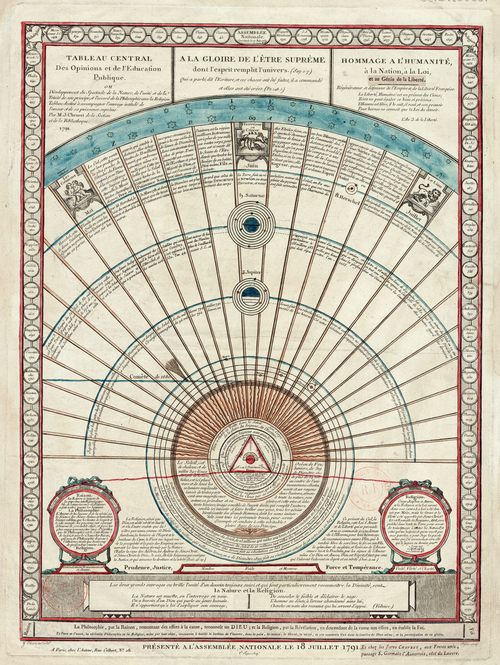
\includegraphics{img/wagner-9.jpg}
\caption*{Abb. 9: Kosmologisch-enzyklopädisches Diagramm mit didaktischer
Funktion, Entwurf von Jean Chevret, gestochen von Jean Baptiste Marie
Poisson, 1791.}
\end{figure}

Chevrets eigene Querverweise zwischen seinen Schriften und dem
\emph{Tableau central des opinions et de l'éducation publique} legen
einen Vergleich zwischen dem Bibliotheks- beziehungsweise Stadtgrundriss
und dem kosmologischen Diagramm nahe. Beide sind radial organisiert und
gehen von einem kreisförmigen Zentrum aus. In diesem befindet sich hier
der alles mit einem Blick überwachende Bibliothekar, dort das nicht
minder wachsame Auge Gottes. Denn Dreieck, Kreis und Halbkreis auf dem
\emph{Tableau central des opinions et de l'éducation publique} können
als ein der christlichen Ikonographie entlehntes, von Chevret auf die
geometrischen Grundformen reduziertes Bildsymbol gelesen werden: das
eines geöffneten Auges, das von einem Dreieck als Zeichen der
Dreifaltigkeit, einer Korona von Lichtstrahlen oder, wie bei Chevret,
gleich von beidem umgeben ist. Bezeichnete dieses Bildsymbol in
christlichem Zusammenhang die Allgegenwart und Allwissenheit Gottes
sowie auch göttliche Vorsehung, dann wurde es im Zuge von Aufklärung und
Französischer Revolution zu einem allsehenden und allwissenden Auge
ebenso des Verstandes wie der republikanischen Legislative
transformiert.\footnote{In dieser Bedeutung führt das Bildsymbol nicht
  nur die Deklaration der Menschen- und Bürgerrechte von 1789 an,
  sondern findet auch in die Vignetten Eingang, die die Dokumente der
  Nationalversammlung und ihrer Abteilungen zieren. Vgl. hierzu Auguste
  Boppe, \emph{Les vignettes emblématiques sous la Révolution}, Paris u.
  Nancy 1911. Zur Transformation dieses Bildsymbols im Kontext der
  Amerikanischen und Französischen Revolution vgl. im Überblick Astrit
  Schmidt-Burkhardt, \enquote{The All-Seer: God's Eye as
  Proto-Surveillance}, in: Thomas Y. Levin (Hg.), \emph{CTRL (space).
  Rhetorics of Surveillance from Bentham to Big Brother}, Karlsruhe u.
  London 2002, S. 17-31.} Die ins absolute räumliche Zentrum der Stadt
Paris und damit der Nation gerückte Bibliothek mit einem Bibliothekar in
ihrer Mitte, der über das Universum des Wissens wacht, kommt dessen
Apotheose nahe. Ein vergleichbares Raum- und Blickdispositiv lässt sich,
wie oben schon angedeutet, für den Hof von Versailles und die
\emph{chambre du roi} rekonstruieren. Als Schnittpunkt aller räumlichen
Achsen war die \emph{chambre du roi} der herausgehobene Ort,
\enquote{von {[}dem{]} aus {[}\ldots{}{]} der Blick beherrschend das
Land und das Leben nach allen Seiten {[}erfasst{]}}.\footnote{Zur Lippe,
  Hof und Schloss des Absolutismus, S. 217.} Rudolf zur Lippe hat in
diesem Zusammenhang nicht nur von einer \enquote{äußerst virulenten
Ambivalenz von Kontrolle und Garantie allgegenwärtiger
Ordnung}\footnote{Ebd., S. 219.} gesprochen. Er hat auch darauf
hingewiesen, dass \enquote{dieser Blick {[}\ldots{}{]} bereits durchaus
etwas von dem panoramatischen Kontrollblick des Aufsehers im Mittelpunkt
jener Gefängnisanlage von Jeremy Bentham {[}hat{]}, die um 1800 aus
bürgerlicher Vorstellung das absolutistische Prinzip für die
geschlossenste aller öffentlichen Anstalten zu einem bestimmten Extrem
steigern sollte}.\footnote{Ebd., S. 218.} In der konkreten Adaptation
dieser Gefängnisarchitektur für den Bibliotheksbau durch Benjamin
Delessert besteht folglich ein letzter konsequenter Schritt.

\subsubsection{Ein Kolosseum, Pantheon und Basar: der Bibliotheksentwurf
Antoine-François
Mauduits}\label{ein-kolosseum-pantheon-und-basar-der-bibliotheksentwurf-antoine-franuxe7ois-mauduits}

Bevor Delessert diesen Schritt 1835 mit seinem ersten von insgesamt zwei
Bibliotheksentwürfen vollzieht, beansprucht Antoine-François Mauduit --
offensichtlich in Reaktion auf die positive Aufnahme von Delesserts
Entwürfen\footnote{Dies zumindest legt der bibliophile Rezensent der
  \emph{Revue générale de l'architecture et des travaux publics} nahe.}
--, das Urheberrecht an einem für die \emph{Place du Carrousel}
geplanten Bibliotheksgebäude mit zentralem Kuppelsaal und strahlenförmig
von ihm ausgehenden Galerien für sich;\footnote{Antoine-François
  Mauduit, \emph{Description d'un projet de bibliothèque composé à Rome
  en 1833, pour la ville de Paris}, Paris 1839.} natürlich fälschlich,
wie der bibliophile Rezensent der \emph{Revue générale de l'architecture
et des travaux publics} mit dem Hinweis auf Chevret betonen wird. Als
strikter Vertreter der \emph{Beaux-arts}-Tradition orientiert sich
Mauduit bei seinem Bibliotheksentwurf an antiken Gebäuden und ihren
Ordnungen.\footnote{\enquote{Überzeugt wie ich davon bin, dass wir noch
  nicht reich genug an Monumenten sind, die an die schönen Zeiten der
  Antike erinnern, um nicht zu versäumen, eine so schöne Gelegenheit zu
  ergreifen, diese Hauptstadt mit etwas Nachahmung dieser schönen
  Modelle zu bereichern, die unsere jungen Künstler in Rom bewundern und
  zeichnen werden, habe ich geplant, mein Gebäude aus drei Ordnungen zu
  bilden, davon für die ersten beiden die dorische und die ionische des
  Marcellustheaters adoptierend. Die dritte Ordnung muss korinthisch
  sein; {[}\ldots{}{]}.} Ebd., S. 8 f.} (Abb. 10) Auf einem Plan macht
sich dieser Entwurf wie folgt aus:\footnote{Bei den in den Pariser
  Bibliotheken vorhandenen Exemplaren von Mauduits Schrift fehlt dieser
  Plan ebenso wie in dem Exemplar der Bayerischen Staatsbibliothek. Der
  hier vorgelegte Plan stammt aus dem Exemplar, das die \emph{National
  Art Library} des Londoner \emph{Victoria and Albert Museum} mit der
  Signatur 503.BB.11 vorhält.} von einer elliptischen Rotunde, die von
einem Kuppeldach überspannt wird und sich \enquote{Panthéon} nennt,
gehen tatsächlich nicht strahlen-, sondern kreuzförmig vier Galerien
aus. Sie münden in einen ebenfalls elliptischen Gebäudering, von Mauduit
als \enquote{Colisée} bezeichnet. Die ellipsoide Form erklärt Mauduit
vom Standort des Bibliotheksgebäudes zwischen Louvre und Tuilerienpalast
her, deren sich nicht treffende Achsen durch das Bibliotheksgebäude
zugleich kaschiert werden sollen. Der Kuppelsaal in der Mitte enthält
als Dekoration die Bilder, Statuen und Büsten auch hier vergangener
Geistesgrößen aus den Künsten und Wissenschaften. An seinen umlaufenden
Wänden sind in doppelwandigen Galerien\footnote{Die aus der Traglast der
  Kuppel resultieren.} Bücher, Antiken und Münzen untergebracht. Nur im
Sommer als Lesesaal dienend,\footnote{Was aus dem Problem der
  Beheizbarkeit dieses Saales und entsprechender Brandgefahr resultiert.}
sieht Mauduit in ihm zugleich einen repräsentativen Ort für
Preisvergaben und Staatsakte. Befindet sich das eigentliche Bücherdepot
in den mittleren Geschossen, so erfüllen Ober- und Erdgeschoss des
Komplexes andere Funktionen. Während Mauduit das von oben beleuchtete
Obergeschoss für die regelmäßigen Kunst- und Industrieausstellungen
öffnet, hat das Erdgeschoss den Zweck, eine Passage zwischen Louvre und
Tuilerienpalast zu bilden. Und es soll in den Arkaden zur \emph{Place du
Carrousel} hin eine Art \enquote{Basar} unterhalten, auf dem jedoch nur
den Wissenschaften und Künsten affine Waren angeboten werden. Im Sinne
Walter Benjamins haben wir es bei dem Bibliotheksentwurf Mauduits mit
einem jener \enquote{Traumhäuser} des 19. Jahrhunderts zu tun, hinter
dessen antiker Hülle bereits die Moderne mit ihrer seriellen
Warenproduktion haust. Der Verkauf der Laden- und Lagerflächen wird denn
auch schon zur spekulativen Gegenfinanzierung der Baukosten für die
Bibliothek in Erwägung gezogen. Die Wohnungen der Bibliotheksverwaltung
bringt Mauduit ebenso wie die der Museumsverwaltung des Louvre in zwei
Stadthäusern in den Ecken der \emph{Place du Carrousel} unter. Mit ihrer
Auslagerung aus dem Bibliotheksgebäude folgt Mauduit einer der
Sicherheitsmaßnahmen gegen Brandgefahr, die sich seit dem späten 18.
Jahrhundert durchzusetzen beginnt. Eine räumlich ähnliche Lösung hatte
Durand für seinen idealtypischen Bibliotheksbau vorgeschlagen. Über die
Verwaltungsräume oder den Ort des Bibliothekars in der Bibliothek selbst
macht Mauduit keine Angaben. Aspekte der Überwachung kommen in diesem
ein französisches Rom herbeisehnenden Entwurf ebenfalls nicht zur
Sprache.

\begin{figure}[htbp]
\centering
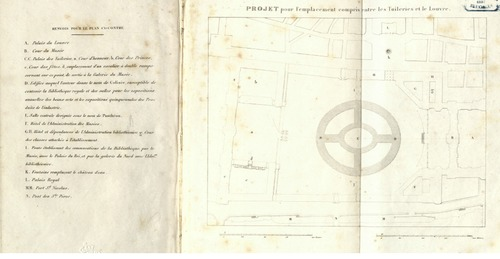
\includegraphics{img/wagner-10.jpg}
\caption*{Abb. 10: Entwurf eines Bibliotheksneubaus für die
\emph{Bibliothèque royale} auf der \emph{Place du Carrousel} von
Antoine-François Mauduit, 1839.}
\end{figure}

\subsubsection{Ein panoptischer Raum: der Bibliotheksentwurf Benjamin
Delesserts}\label{ein-panoptischer-raum-der-bibliotheksentwurf-benjamin-delesserts}

Dafür erscheinen sie für die \enquote{forme panoptique} konstitutiv, die
Benjamin Delessert seinen beiden Bibliotheksentwürfen von 1835 und 1838
zugrunde legt. Während sich der erste auf die \emph{Place du Carrousel}
bezieht und als Rundbau angelegt ist, reagiert der zweite für die
\emph{Place de Bellechasse} auf diesen Standort mit einer Stauchung der
Rotunde zu einem Oval, das von einem rechteckigen Baukörper mit Portikus
ummantelt wird.\footnote{Beide Plätze wurden in den 1830er Jahren als
  mögliche Standorte eines Neubaus für die \emph{Bibliothèque royale}
  gehandelt.} Obwohl Delessert weder Architekt noch Bibliothekar ist,
gesteht ihm der bibliophile Rezensent der \emph{Revue générale de
l'architecture et des travaux publics} zu, aufgrund seiner Erfahrungen,
die er als Besitzer einer der umfangreichsten naturkundlichen
Bibliotheken des 19. Jahrhunderts gesammelt hat, gleichsam die
\enquote{Sprache der Bibliothek} zu sprechen.\footnote{Anonymus, La
  Bibliothèque royale, S. 309. Wie Delessert in seinem \emph{Mémoire}
  von 1835 zu verstehen gibt, bot ihm seine eigene Sammlung tatsächlich
  Anlass, über die beste Anordnung, die man einer Bibliothek geben kann,
  nachzudenken.} Doch Delessert spricht nicht nur als Sammler, sondern
auch als Bankier und Industrieller. Hebt er doch an seinen Entwürfen vor
allem deren Ökonomie hervor.\footnote{Was auch die Baukosten und die
  Bauzeit einbezieht.} So soll das für 800.000 Bände geplante
Bibliotheksgebäude, wenn es als Rundbau beziehungsweise Oval ausgeführt
wird, deutlich weniger Raum einnehmen als ein länglicher Baukörper,
unabhängig davon, ob jener als durchgehendes Gebäude oder auf dem
Grundriss eines griechischen Kreuzes mit Höfen angelegt ist. Delessert
unterstreicht das auf seinem Bibliotheksplan durch einen visuellen
Vergleich der entsprechenden Flächenausdehnungen. (Abb. 11)

\begin{figure}[htbp]
\centering
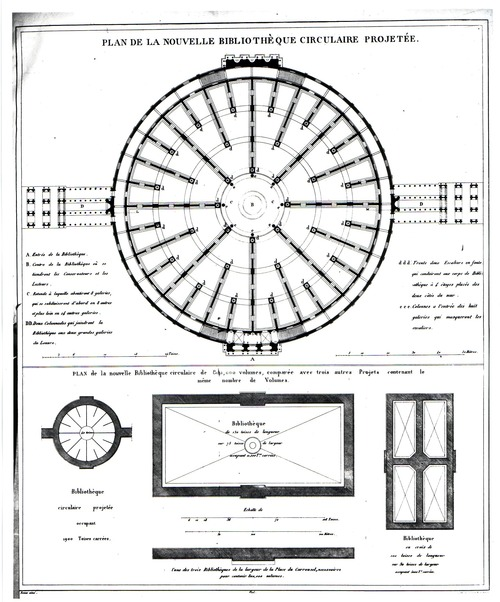
\includegraphics{img/wagner-11.jpg}
\caption*{Abb. 11: Entwurf eines Bibliotheksneubaus für die
\emph{Bibliothèque royale} auf der \emph{Place du Carrousel} von
Benjamin Delessert, 1835.}
\end{figure}

Über die Mitte seines Bibliotheksrundbaus erhebt sich ein Tambour, der
an Stelle einer Kuppel ein Zeltdach aufweist. Von außen ist er mit einem
Figurenfries verkleidet, sodass der Lichteinfall ausschließlich durch
die seitlichen Fensteröffnungen der Rotunde kommt.\footnote{In seinem
  zweiten Bibliotheksentwurf von 1838, bei dem er die \enquote{forme
  panoptique} an die \emph{Place de Bellechasse} als neudiskutierten
  Standort der Bibliothek anpasst, indem er den Rundbau zu einem
  ummantelten Oval werden lässt, sieht Delessert hingegen Oberlicht vor.
  Vgl. Benjamin Delessert, \emph{Second mémoire sur la Bibliothèque
  Royale sur l'emplacement ou elle pourrait être construite, et sur la
  meilleure disposition à donner aux grandes bibliothèques publiques},
  Paris 1838.} Acht den Tambour tragende Säulen korinthischer Ordnung
umlaufen den zentralen Saal im Inneren der Bibliothek. Von ihnen gehen
radial acht Wände aus. Zwischen diesen sind jeweils noch einmal drei
Wände unterschiedlicher Länge eingefügt. Alle Wände erstrecken sich über
die gesamte Höhe des Raumes und sind beidseitig mit in Eisen
ausgeführten Galerien und Büchergestellen versehen. Zugang zu den
Galerien und Sammlungsbeständen erfolgt über gusseiserne Wendeltreppen.
Rund zehn Jahre, bevor eine Eisenkonstruktion mit Labroustes Bibliothek
\emph{Sainte-Geneviève} in den Bibliotheksbau Einzug hält, nimmt
Delessert sie hier vorweg. Sieht Delessert für seinen ersten Entwurf von
1835 noch vor, die gusseisernen Treppen hinter klassizistischen Säulen
zu verstecken, dann sind in dem zweiten Entwurf von 1838 auch die
Säulen, die den zentralen Saal einfassen, in Gusseisen ausgeführt. Die
avancierte Verwendung des neuen Baumaterials verbleibt bei Delessert
jedoch hinter einer klassizistischen Verkleidung der Gebäude nach außen;
für Benjamin tritt die Moderne auch hinsichtlich der Baumaterialien in
antiker Entstellung auf. Die räumliche Anordnung der Bestände verspricht
zugleich eine ökonomische Beschaffung der an den Wänden zum Teil in
Glasschränken verwahrten Bücher. Weder sind Lesesaal und Magazin
räumlich voneinander getrennt, noch gibt es lange Beschaffungswege wie
etwa bei einer Enfilade von Büchersälen. Vom räumlichen Mittelpunkt aus,
an dem sich die Bibliothekare und die Aufseher (\enquote{gardiens})
befinden, sind alle Wege in alle Richtungen gleich begrenzt. Die
Kreissegmente, gebildet durch die radial vom Zentrum ausgehenden Mauern,
dienen hierbei der systematischen Aufstellung der Buchbestände. Ihnen
sind an Klassen zugeordnet: Theologie, Jurisprudenz, Administration,
Handel und Finanzen, Naturgeschichte, Wissenschaften und Künste,
Literatur, Geschichte, Reisen.

Aus der Position des obersten Bibliothekars in der absoluten Mitte des
Raumes leitet sich schließlich eine Ökonomie der Überwachung her. Denn
von seinem zentralen Standort kann er mit \enquote{einem Blick die
Galerien bis an ihr Ende überblicken und alle dort sich bewegenden
Personen sehen}.\footnote{Delessert, Second mémoire sur la Bibliothèque
  Royale, S. 4.} Auf diese Weise hätte er neben allen Bediensteten auch
die 500 Leser, die in dem Saal Platz finden sollen, jederzeit unter
Kontrolle; wobei Delessert zur Ausrichtung der Lesepulte keine näheren
Angaben macht. In dieser räumlichen Disposition der Bibliothek besteht
ihre \enquote{forme panoptique}. Unmittelbares Vorbild, das Delessert
indessen nicht benennt, ist Jeremy Benthams Panopticon: vorgesehen für
überhaupt alle Gebäude, in denen eine größere Menge an Menschen zu
\enquote{verwalten} ist, wie Krankenhaus, Asyl oder Schule, nehmen die
Insassen des Panopticons in ihren Zellen den äußeren Ring eines Rundbaus
ein. Überwacht werden sie vom Gefängniswärter, dessen Beobachtungsturm
in der Mitte des Gebäudes so eingerichtet ist, dass ein asymmetrisches
Sichtverhältnis besteht. Während der Wärter alle Insassen sehen kann,
können diese nicht erkennen, ob sie gerade von ihm beobachtet werden.
Weil sie dieses aber nicht können, werden sie sich jederzeit so
verhalten, als ob sie unter Beobachtung stünden, nämlich regelkonform,
so zumindest die Annahme Benthams.\footnote{Vgl. Bentham, Panopticon; or
  the inspection-house.}

Delessert hat diese Quelle nicht genannt.\footnote{Für Delesserts eigene
  Kenntnis des Panopticons kommen mehrere Kanäle in Frage. Zum einen ist
  hier die französische Ausgabe von Benthams Schrift zu nennen. Vgl.
  Jérémie Bentham, \emph{Panoptique. Mémoire sur un nouveau principe
  pour construire des maisons d'inspection et nommément des maisons de
  force; imprimé par ordre de l'Assemblée Nationale}, Paris 1791. Zum
  anderen wurde der Vater Benjamin Delesserts, Étienne Delessert, 1790
  als Übersetzer einer finanzökonomischen Schrift Benthams tätig. Der
  Neffe Jeremy Benthams, der Botaniker George Bentham, besuchte in den
  1830er Jahren wiederum Delesserts Herbarium in Paris. Es bestanden
  damit direkte Beziehungen zwischen den Familien Bentham und Delessert.}
Als Vorbild seiner Rotunde für die \emph{Place du Carrousel} zwischen
Louvre und Tuilerienpalast führt Delessert lediglich eine von
Louis-Pierre Baltard für diesen Standort entworfene Orangerie
an.\footnote{Hintergrund von Baltards Entwurf waren zwei von der
  Regierung unter Napoleon ausgeschriebene Wettbewerbe: 1807 für eine
  Orangerie für die \emph{Place du Carrousel} und 1810 für eine
  Verbindung zwischen Louvre und Tuilerienpalast, für die neben Baltards
  Orangerie offensichtlich auch andere Rundbauten entworfen wurden.
  Mauduits und Delesserts Bibliotheksbauten schließen in ihrer
  Konzeption an diese Platzgestaltung durch einen, die verschiedenen
  Achsen von Louvre und Tuilerienpalast überspielenden Rundbau an. Vgl.
  hierzu Pierre Pinon, \emph{Louis-Pierre et Victor Baltard}, Paris
  2005, S. 23-25.} Konnte er also davon ausgehen, dass die Anleihe der
\enquote{forme panoptique} bei Benthams Panopticon in den 1830er Jahren
so deutlich war, dass sie nicht eigens erwähnt werden musste? Immerhin
lag Benthams entsprechende Schrift seit 1791 in französischer
Übersetzung vor.\footnote{Jérémie Bentham, Panoptique.} Oder wollte er
die Beziehung seines Bibliotheksentwurfs zu einer Gefängnisarchitektur
nicht weiter herausstellen? Die breite Rezeption seiner Entwürfe
jedenfalls hat dieser Beziehung kaum Beachtung geschenkt. Schon Laborde,
über dessen achten Brief zur Konstruktion von Bibliotheken insbesondere
Delesserts erster Bibliotheksentwurf von 1835 in die Geschichte der
Bibliotheksarchitektur Einzug gehalten hat, weist mit keinem Wort auf
das Vorbild der \enquote{forme panoptique} hin. Wohl aber kritisiert er
die räumliche Disposition von Delesserts \enquote{surveillance
complète}.\footnote{Delessert, Mémoire sur la Bibliothèque Royale, S. 4.}
Denn um sie realisieren zu können, müsste sich der oberste Bibliothekar
nicht nur \enquote{beständig um eine bewegliche Achse drehen}, er müsste
auch \enquote{mit einem Fernrohr und einem Sprachrohr}\footnote{Laborde,
  Étude sur la Construction des Bibliothèques, S. 35.} ausgestattet
sein. Und was für die Repräsentation des absolutistischen Herrschers
noch Sinn macht, dass alle räumlichen Linien in nur einem Punkt, dem von
ihm eingenommenen Punkt (der \emph{chambre du roi}),
zentralperspektivisch zusammenlaufen, erweist sich für die Bibliothek
als Nachteil. Laborde erkennt: \enquote{{[}\ldots{}{]} und wie es nur
einer Person gegeben ist, sich mitten im Zentrum zu platzieren, ist die
Sicht für alle anderen noch weit ungünstiger, denn außerhalb dieses
Zentrums der Konvergenz ist nicht mehr als eine Unordnung der Linien und
der Regale, ohne irgendeine Regularität der Perspektive}.\footnote{Ebd.}
Labordes Kritik an den Bibliotheksentwürfen von Delessert wird in der
Folge vielfach übernommen. Es steht dabei jedoch weniger die
\enquote{forme panoptique} zur Disposition als der Rundbau als solcher,
den Laborde -- entgegen Delesserts Argumentation -- ebenfalls für
vollkommen unökonomisch hält. Eine Verbindung zu Benthams Panopticon
wird also auch nach Laborde nicht hergestellt. Eine Ausnahme bilden
Edward Edwards \emph{Memoirs of Libraries} aus der Mitte des 19.
Jahrhunderts sowie ein Beitrag aus der jüngeren Historiographie der
Bibliothek.\footnote{Edwards schreibt: \enquote{Many years ago, the late
  M. Benjamin Delessert, distinguished both as a Member of the Chamber
  of Deputies, and as a botanist (and himself the collector of some
  30,000 volumes of well-chosen books,) recommended the construction of
  a new building for the same Library, on that \enquote{panopticon}
  principle, the application of which to prisons was so enthusiastically
  advocated by Bentham.} Edward Edwards\emph{, Memoirs of Libraries:
  including a Handbook of library economy}, Vol. 1, London 1859, S. 712.
  Während Jean-François Foucaud lapidar feststellt, dass Delessert
  Bentham gelesen hat. Jean-François Foucaud, \enquote{Extensions et
  travaux de la Bibliothèque nationale}, in: \emph{Histoire de les
  Bibliothèques francaises}, tome 3: \enquote{Les bibliothèques de la
  Révolution et du XIX siècle}, Paris 2009, S. 335-355, hier S. 340. Zur
  allgemeinen Rezeption des Panopticons in der Bibliotheksarchitektur
  des 19. Jahrhunderts, jedoch ohne Hinweis auf Delessert, vgl. Alistair
  Black, Simon Pepper u. Kaye Bagshaw, \emph{Books, Buildings and Social
  Engineering. Early Public Libraries in Britain from Past to Present},
  Farnham, Surrey u.a. 2009, S. 42-70.} Das heißt nicht, dass Delesserts
Entwurf beziehungsweise die \enquote{forme panoptique} keine Wirkung
gehabt hätte. Bis zum Ende des 19. Jahrhunderts und darüber hinaus
entstanden neben weiteren panoptischen Bibliotheksentwürfen mehrere
Kuppellesesäle, bei denen sich im Zentrum die bibliothekarische Aufsicht
und der Katalog befanden. Die Anordnung der Lesepulte folgte in diesen
Bibliotheken entweder einem radialen System wie im Lesesaal des
\emph{British Museum} (1854-1856) und der \emph{Manchester Central
Library} (1930-1934) oder einem zirkulären wie in der \emph{Congress
Library} in Washington (1886-1897). Der \enquote{circular reading room}
galt als \enquote{ideal library space}, wo es um die Überwachung sowohl
der Bibliotheksnutzer wie auch der Bibliotheksangestellten
ging.\footnote{Ebd., S. 52.}

\subsubsection{Epilog: Verkörperungen des panoptischen Blickregimes,
oder die Büste des Souveräns im Zentrum der
Bibliothek}\label{epilog-verkuxf6rperungen-des-panoptischen-blickregimes-oder-die-buxfcste-des-souveruxe4ns-im-zentrum-der-bibliothek}

Am Überwachungsturm des Panopticons, der seine Funktion auch dann
erfüllt, wenn er nicht durch den Gefängniswärter besetzt ist, hat Michel
Foucault seine These veranschaulicht, dass die moderne Disziplin kein
souveränes Subjekt mehr voraussetzt, das die Macht auf sich versammelt
und für alle sichtbar ausübt.\footnote{Vgl. hierzu Michel Foucault,
  \emph{Überwachen und Strafen. Die Geburt des Gefängnisses} (frz.
  1975), Frankfurt/M. 1994.} Die Disziplin folgt einer anderen Logik.
Sie ist über die gesamte Gesellschaft und ihre Institutionen verteilt
und beruht auf der Verinnerlichung räumlich strukturierter
Verhaltensregeln. Für die panoptischen Bibliotheksentwürfe gilt das so
nicht. Der Bibliothekar, der bei Chevret anstelle des absolutistischen
Herrschers in das perspektivische Zentrum des (Bibliotheks)Raumes
einrückt, bleibt dort auch bei Delessert. (Abb. 12) Und selbst Laborde,
der Delessert einer radikalen Kritik unterzieht, wird das Zentrum seiner
eigenen Bibliotheksentwürfe nicht leer lassen. Zwar wird das Zentrum
seiner Bibliothek auf kreuzförmigem Grundriss nur von einer kleinen
Kuppel bekrönt, doch befinden sich auch dort, im Karree um den Katalog
herum angeordnet, die leicht erhöhten Pulte der Bibliothekare, von denen
sich die in den Querarmen aufgestellten Lesepulte überwachen lassen. Das
eigentliche räumliche wie panoptische Zentrum der Bibliothek wird bei
Laborde jedoch weder durch die Aufsicht führenden und Buchbestellungen
entgegennehmenden Bibliothekare gebildet noch durch den Katalog, sondern
durch eine Büste des Souveräns, die Laborde oben auf dem kreisrunden
Kataloggestell untergebracht hat. Der Souverän nimmt damit noch einmal
(und dies bis zum Ende der Julimonarchie) den idealen
Betrachterstandpunkt ein. Mit seiner imaginären Anwesenheit beherrscht
er nicht nur den Lesesaal, im übertragenen Sinne beherrscht er auch die
Bibliothek als inzwischen nationale Institution des Wissens und
Gedächtnisses. Der Katalog als Verweisungssystem, über das auf den
materiellen Buchbestand zugegriffen wird, ist darüber buchstäblich zum
Körper des Souveräns geworden.

\begin{figure}[htbp]
\centering
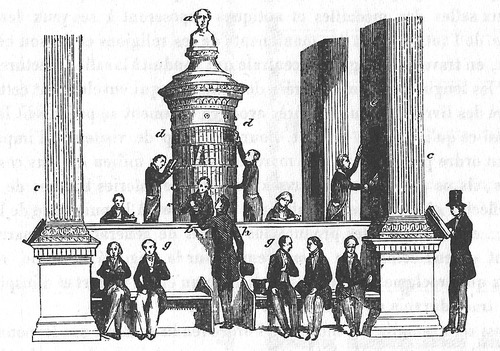
\includegraphics{img/wagner-12.jpg}
\caption*{Abb. 12: Bibliothekskatalog mit Büste des Souveräns nach Léon
de Laborde, 1845.}
\end{figure}

Wie die ausgehend von der \emph{Revue générale de l'architecture et des
travaux publics} rekonstruierte Bibliotheksdiskussion in der ersten
Hälfte des 19. Jahrhunderts gezeigt hat, vollzog sich der Übergang von
der barocken Saalbibliothek zur modernen Magazinbibliothek nicht linear.
Die zahlreichen Entwürfe und Anschlüsse an andere Gebäudetypen zeigen,
dass sowohl die Ausdehnung der Gutenberggalaxis im 19. Jahrhundert als
auch die neuen Funktionen der Bibliothek für einen neuen Nutzerkreis
zuallererst reflexiv werden mussten, um darauf eine architektonische
Antwort finden zu können. Einige dieser Antworten haben Bestand gehabt,
andere nicht. Dem bibliophilen Rezensenten der \emph{Revue générale de
l'architecture et des travaux publics} bleibt abschließend zu sagen,
dass Mauduit und Delessert nicht auf Chevret zurückgreifen mussten (und
dieses wohl auch nicht getan haben), damit sie zu ihren
Bibliotheksrundbauten kommen konnten. Sein Verdienst bleibt es, mit dem
Hinweis auf Chevrets Bibliotheksentwurf einen Moment in der
Bibliotheksgeschichte festgehalten zu haben, als sich in die
Bibliotheksrotunde, Symbol eines enzyklopädischen, universalen Wissens,
die Idee eines Blickregimes einschreibt, das von Bentham panoptisch
genannt worden ist. 
